\documentclass[1p]{elsarticle_modified}
%\bibliographystyle{elsarticle-num}

%\usepackage[colorlinks]{hyperref}
%\usepackage{abbrmath_seonhwa} %\Abb, \Ascr, \Acal ,\Abf, \Afrak
\usepackage{amsfonts}
\usepackage{amssymb}
\usepackage{amsmath}
\usepackage{amsthm}
\usepackage{scalefnt}
\usepackage{amsbsy}
\usepackage{kotex}
\usepackage{caption}
\usepackage{subfig}
\usepackage{color}
\usepackage{graphicx}
\usepackage{xcolor} %% white, black, red, green, blue, cyan, magenta, yellow
\usepackage{float}
\usepackage{setspace}
\usepackage{hyperref}

\usepackage{tikz}
\usetikzlibrary{arrows}

\usepackage{multirow}
\usepackage{array} % fixed length table
\usepackage{hhline}

%%%%%%%%%%%%%%%%%%%%%
\makeatletter
\renewcommand*\env@matrix[1][\arraystretch]{%
	\edef\arraystretch{#1}%
	\hskip -\arraycolsep
	\let\@ifnextchar\new@ifnextchar
	\array{*\c@MaxMatrixCols c}}
\makeatother %https://tex.stackexchange.com/questions/14071/how-can-i-increase-the-line-spacing-in-a-matrix
%%%%%%%%%%%%%%%

\usepackage[normalem]{ulem}

\newcommand{\msout}[1]{\ifmmode\text{\sout{\ensuremath{#1}}}\else\sout{#1}\fi}
%SOURCE: \msout is \stkout macro in https://tex.stackexchange.com/questions/20609/strikeout-in-math-mode

\newcommand{\cancel}[1]{
	\ifmmode
	{\color{red}\msout{#1}}
	\else
	{\color{red}\sout{#1}}
	\fi
}

\newcommand{\add}[1]{
	{\color{blue}\uwave{#1}}
}

\newcommand{\replace}[2]{
	\ifmmode
	{\color{red}\msout{#1}}{\color{blue}\uwave{#2}}
	\else
	{\color{red}\sout{#1}}{\color{blue}\uwave{#2}}
	\fi
}

\newcommand{\Sol}{\mathcal{S}} %segment
\newcommand{\D}{D} %diagram
\newcommand{\A}{\mathcal{A}} %arc


%%%%%%%%%%%%%%%%%%%%%%%%%%%%%5 test

\def\sl{\operatorname{\textup{SL}}(2,\Cbb)}
\def\psl{\operatorname{\textup{PSL}}(2,\Cbb)}
\def\quan{\mkern 1mu \triangleright \mkern 1mu}

\theoremstyle{definition}
\newtheorem{thm}{Theorem}[section]
\newtheorem{prop}[thm]{Proposition}
\newtheorem{lem}[thm]{Lemma}
\newtheorem{ques}[thm]{Question}
\newtheorem{cor}[thm]{Corollary}
\newtheorem{defn}[thm]{Definition}
\newtheorem{exam}[thm]{Example}
\newtheorem{rmk}[thm]{Remark}
\newtheorem{alg}[thm]{Algorithm}

\newcommand{\I}{\sqrt{-1}}
\begin{document}

%\begin{frontmatter}
%
%\title{Boundary parabolic representations of knots up to 8 crossings}
%
%%% Group authors per affiliation:
%\author{Yunhi Cho} 
%\address{Department of Mathematics, University of Seoul, Seoul, Korea}
%\ead{yhcho@uos.ac.kr}
%
%
%\author{Seonhwa Kim} %\fnref{s_kim}}
%\address{Center for Geometry and Physics, Institute for Basic Science, Pohang, 37673, Korea}
%\ead{ryeona17@ibs.re.kr}
%
%\author{Hyuk Kim}
%\address{Department of Mathematical Sciences, Seoul National University, Seoul 08826, Korea}
%\ead{hyukkim@snu.ac.kr}
%
%\author{Seokbeom Yoon}
%\address{Department of Mathematical Sciences, Seoul National University, Seoul, 08826,  Korea}
%\ead{sbyoon15@snu.ac.kr}
%
%\begin{abstract}
%We find all boundary parabolic representation of knots up to 8 crossings.
%
%\end{abstract}
%\begin{keyword}
%    \MSC[2010] 57M25 
%\end{keyword}
%
%\end{frontmatter}

%\linenumbers
%\tableofcontents
%
\newcommand\colored[1]{\textcolor{white}{\rule[-0.35ex]{0.8em}{1.4ex}}\kern-0.8em\color{red} #1}%
%\newcommand\colored[1]{\textcolor{white}{ #1}\kern-2.17ex	\textcolor{white}{ #1}\kern-1.81ex	\textcolor{white}{ #1}\kern-2.15ex\color{red}#1	}

{\Large $\underline{12a_{1020}~(K12a_{1020})}$}

\setlength{\tabcolsep}{10pt}
\renewcommand{\arraystretch}{1.6}
\vspace{1cm}\begin{tabular}{m{100pt}>{\centering\arraybackslash}m{274pt}}
\multirow{5}{120pt}{
	\centering
	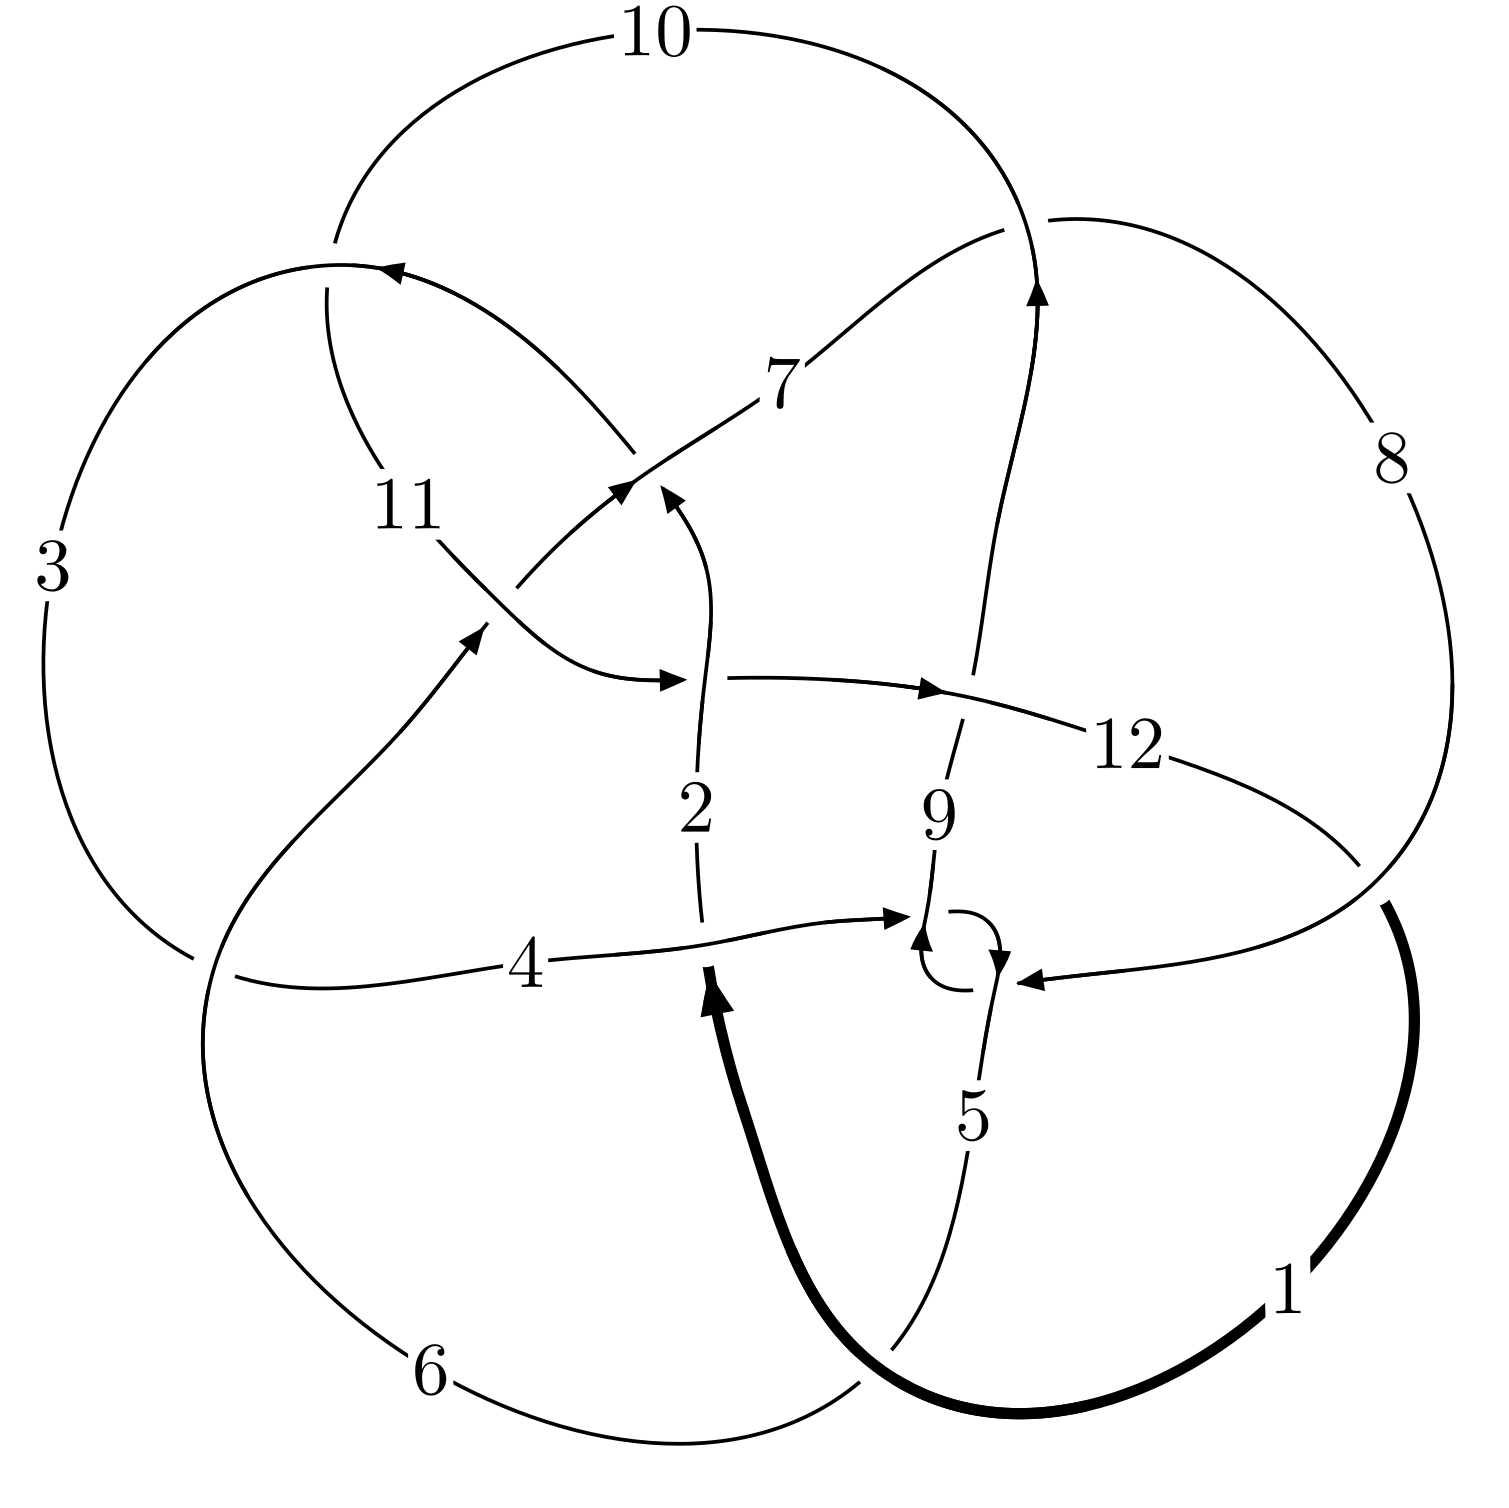
\includegraphics[width=112pt]{../../../GIT/diagram.site/Diagrams/png/1821_12a_1020.png}\\
\ \ \ A knot diagram\footnotemark}&
\allowdisplaybreaks
\textbf{Linearized knot diagam} \\
\cline{2-2}
 &
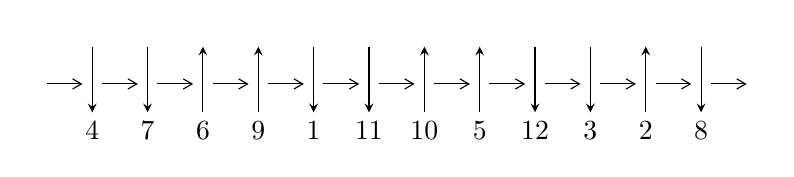
\begin{tikzpicture}[x=20pt, y=17pt]
	% nodes
	\node (C0) at (0, 0) {};
	\node (C1) at (1, 0) {};
	\node (C1U) at (1, +1) {};
	\node (C1D) at (1, -1) {4};

	\node (C2) at (2, 0) {};
	\node (C2U) at (2, +1) {};
	\node (C2D) at (2, -1) {7};

	\node (C3) at (3, 0) {};
	\node (C3U) at (3, +1) {};
	\node (C3D) at (3, -1) {6};

	\node (C4) at (4, 0) {};
	\node (C4U) at (4, +1) {};
	\node (C4D) at (4, -1) {9};

	\node (C5) at (5, 0) {};
	\node (C5U) at (5, +1) {};
	\node (C5D) at (5, -1) {1};

	\node (C6) at (6, 0) {};
	\node (C6U) at (6, +1) {};
	\node (C6D) at (6, -1) {11};

	\node (C7) at (7, 0) {};
	\node (C7U) at (7, +1) {};
	\node (C7D) at (7, -1) {10};

	\node (C8) at (8, 0) {};
	\node (C8U) at (8, +1) {};
	\node (C8D) at (8, -1) {5};

	\node (C9) at (9, 0) {};
	\node (C9U) at (9, +1) {};
	\node (C9D) at (9, -1) {12};

	\node (C10) at (10, 0) {};
	\node (C10U) at (10, +1) {};
	\node (C10D) at (10, -1) {3};

	\node (C11) at (11, 0) {};
	\node (C11U) at (11, +1) {};
	\node (C11D) at (11, -1) {2};

	\node (C12) at (12, 0) {};
	\node (C12U) at (12, +1) {};
	\node (C12D) at (12, -1) {8};
	\node (C13) at (13, 0) {};

	% arrows
	\draw[->,>={angle 60}]
	(C0) edge (C1) (C1) edge (C2) (C2) edge (C3) (C3) edge (C4) (C4) edge (C5) (C5) edge (C6) (C6) edge (C7) (C7) edge (C8) (C8) edge (C9) (C9) edge (C10) (C10) edge (C11) (C11) edge (C12) (C12) edge (C13) ;	\draw[->,>=stealth]
	(C1U) edge (C1D) (C2U) edge (C2D) (C3D) edge (C3U) (C4D) edge (C4U) (C5U) edge (C5D) (C6U) edge (C6D) (C7D) edge (C7U) (C8D) edge (C8U) (C9U) edge (C9D) (C10U) edge (C10D) (C11D) edge (C11U) (C12U) edge (C12D) ;
	\end{tikzpicture} \\
\hhline{~~} \\& 
\textbf{Solving Sequence} \\ \cline{2-2} 
 &
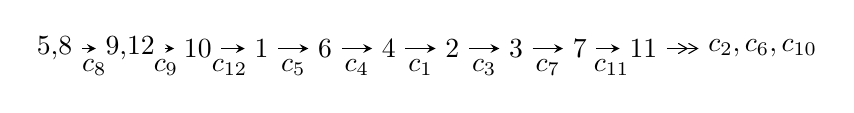
\begin{tikzpicture}[x=23pt, y=7pt]
	% node
	\node (A0) at (-1/8, 0) {5,8};
	\node (A1) at (17/16, 0) {9,12};
	\node (A2) at (17/8, 0) {10};
	\node (A3) at (25/8, 0) {1};
	\node (A4) at (33/8, 0) {6};
	\node (A5) at (41/8, 0) {4};
	\node (A6) at (49/8, 0) {2};
	\node (A7) at (57/8, 0) {3};
	\node (A8) at (65/8, 0) {7};
	\node (A9) at (73/8, 0) {11};
	\node (C1) at (1/2, -1) {$c_{8}$};
	\node (C2) at (13/8, -1) {$c_{9}$};
	\node (C3) at (21/8, -1) {$c_{12}$};
	\node (C4) at (29/8, -1) {$c_{5}$};
	\node (C5) at (37/8, -1) {$c_{4}$};
	\node (C6) at (45/8, -1) {$c_{1}$};
	\node (C7) at (53/8, -1) {$c_{3}$};
	\node (C8) at (61/8, -1) {$c_{7}$};
	\node (C9) at (69/8, -1) {$c_{11}$};
	\node (A10) at (11, 0) {$c_{2},c_{6},c_{10}$};

	% edge
	\draw[->,>=stealth]	
	(A0) edge (A1) (A1) edge (A2) (A2) edge (A3) (A3) edge (A4) (A4) edge (A5) (A5) edge (A6) (A6) edge (A7) (A7) edge (A8) (A8) edge (A9) ;
	\draw[->>,>={angle 60}]	
	(A9) edge (A10);
\end{tikzpicture} \\ 

\end{tabular} \\

\footnotetext{
The image of knot diagram is generated by the software ``\textbf{Draw programme}" developed by Andrew Bartholomew(\url{http://www.layer8.co.uk/maths/draw/index.htm\#Running-draw}), where we modified some parts for our purpose(\url{https://github.com/CATsTAILs/LinksPainter}).
}\phantom \\ \newline 
\centering \textbf{Ideals for irreducible components\footnotemark of $X_{\text{par}}$} 
 
\begin{align*}
I^u_{1}&=\langle 
-5.40044\times10^{30} u^{51}-1.18633\times10^{32} u^{50}+\cdots+1.35700\times10^{31} b+1.73576\times10^{33},\\
\phantom{I^u_{1}}&\phantom{= \langle  }-2.27295\times10^{32} u^{51}-4.78994\times10^{33} u^{50}+\cdots+2.98541\times10^{32} a-2.85705\times10^{35},\\
\phantom{I^u_{1}}&\phantom{= \langle  }u^{52}+19 u^{51}+\cdots+4304 u+352\rangle \\
I^u_{2}&=\langle 
6.44508\times10^{84} a u^{75}-2.08267\times10^{91} u^{75}+\cdots-3.22254\times10^{84} a+1.52479\times10^{91},\\
\phantom{I^u_{2}}&\phantom{= \langle  }-1.34824\times10^{87} a u^{75}+5.19629\times10^{86} u^{75}+\cdots+2.29637\times10^{87} a-2.56035\times10^{87},\\
\phantom{I^u_{2}}&\phantom{= \langle  }2 u^{76}-21 u^{75}+\cdots+7 u+1\rangle \\
I^u_{3}&=\langle 
-33715462178301 u^{32}-249975325620775 u^{31}+\cdots+13110454304539 b-1988240417047,\\
\phantom{I^u_{3}}&\phantom{= \langle  }-31727221761254 u^{32}-267784864462700 u^{31}+\cdots+13110454304539 a-56379097685388,\\
\phantom{I^u_{3}}&\phantom{= \langle  }u^{33}+8 u^{32}+\cdots-2 u+1\rangle \\
I^u_{4}&=\langle 
2 u^5 a-3 u^4 a-4 u^5+6 u^3 a+6 u^4-3 u^2 a-12 u^3+4 a u+8 u^2+b- a-9 u+3,\\
\phantom{I^u_{4}}&\phantom{= \langle  }-2 u^5 a+5 u^4 a-2 u^5-11 u^3 a+3 u^4+10 u^2 a+a^2-8 a u-6 u^2+a+8 u-2,\\
\phantom{I^u_{4}}&\phantom{= \langle  }2 u^6-5 u^5+9 u^4-9 u^3+7 u^2-4 u+1\rangle \\
\\
\end{align*}
\raggedright * 4 irreducible components of $\dim_{\mathbb{C}}=0$, with total 249 representations.\\
\footnotetext{All coefficients of polynomials are rational numbers. But the coefficients are sometimes approximated in decimal forms when there is not enough margin.}
\newpage
\renewcommand{\arraystretch}{1}
\centering \section*{I. $I^u_{1}= \langle -5.40\times10^{30} u^{51}-1.19\times10^{32} u^{50}+\cdots+1.36\times10^{31} b+1.74\times10^{33},\;-2.27\times10^{32} u^{51}-4.79\times10^{33} u^{50}+\cdots+2.99\times10^{32} a-2.86\times10^{35},\;u^{52}+19 u^{51}+\cdots+4304 u+352 \rangle$}
\flushleft \textbf{(i) Arc colorings}\\
\begin{tabular}{m{7pt} m{180pt} m{7pt} m{180pt} }
\flushright $a_{5}=$&$\begin{pmatrix}0\\u\end{pmatrix}$ \\
\flushright $a_{8}=$&$\begin{pmatrix}1\\0\end{pmatrix}$ \\
\flushright $a_{9}=$&$\begin{pmatrix}1\\- u^2\end{pmatrix}$ \\
\flushright $a_{12}=$&$\begin{pmatrix}0.761351 u^{51}+16.0445 u^{50}+\cdots+10398.7 u+957.005\\0.397967 u^{51}+8.74225 u^{50}+\cdots-479.088 u-127.911\end{pmatrix}$ \\
\flushright $a_{10}=$&$\begin{pmatrix}-2.70304 u^{51}-46.8969 u^{50}+\cdots-3895.42 u-399.652\\2.93589 u^{51}+57.3067 u^{50}+\cdots+21884.4 u+1984.90\end{pmatrix}$ \\
\flushright $a_{1}=$&$\begin{pmatrix}0.363384 u^{51}+7.30226 u^{50}+\cdots+10877.8 u+1084.92\\0.397967 u^{51}+8.74225 u^{50}+\cdots-479.088 u-127.911\end{pmatrix}$ \\
\flushright $a_{6}=$&$\begin{pmatrix}0.908460 u^{51}+16.5220 u^{50}+\cdots+24384.8 u+2445.30\\-0.738720 u^{51}-8.56649 u^{50}+\cdots-1463.71 u-319.778\end{pmatrix}$ \\
\flushright $a_{4}=$&$\begin{pmatrix}- u\\u^3+u\end{pmatrix}$ \\
\flushright $a_{2}=$&$\begin{pmatrix}0.105046 u^{51}+0.592168 u^{50}+\cdots+4488.89 u+506.488\\-1.38508 u^{51}-24.8619 u^{50}+\cdots-1935.50 u-183.673\end{pmatrix}$ \\
\flushright $a_{3}=$&$\begin{pmatrix}4.68723 u^{51}+81.2745 u^{50}+\cdots+19555.9 u+1971.13\\-6.25802 u^{51}-115.562 u^{50}+\cdots-28852.9 u-2683.34\end{pmatrix}$ \\
\flushright $a_{7}=$&$\begin{pmatrix}-2.09264 u^{51}-37.0957 u^{50}+\cdots+3061.71 u+351.415\\2.83123 u^{51}+55.6059 u^{50}+\cdots+21975.9 u+1963.10\end{pmatrix}$ \\
\flushright $a_{11}=$&$\begin{pmatrix}3.82698 u^{51}+70.5532 u^{50}+\cdots+34625.1 u+3353.24\\-2.85778 u^{51}-49.9394 u^{50}+\cdots-7240.73 u-763.558\end{pmatrix}$\\&\end{tabular}
\flushleft \textbf{(ii) Obstruction class $= -1$}\\~\\
\flushleft \textbf{(iii) Cusp Shapes $= -6.09524 u^{51}-97.4706 u^{50}+\cdots+31667.1 u+2690.77$}\\~\\
\newpage\renewcommand{\arraystretch}{1}
\flushleft \textbf{(iv) u-Polynomials at the component}\newline \\
\begin{tabular}{m{50pt}|m{274pt}}
Crossings & \hspace{64pt}u-Polynomials at each crossing \\
\hline $$\begin{aligned}c_{1},c_{9}\end{aligned}$$&$\begin{aligned}
&u^{52}+u^{51}+\cdots-52 u^3+4
\end{aligned}$\\
\hline $$\begin{aligned}c_{2},c_{6}\end{aligned}$$&$\begin{aligned}
&u^{52}-3 u^{50}+\cdots-3 u+1
\end{aligned}$\\
\hline $$\begin{aligned}c_{3},c_{7}\end{aligned}$$&$\begin{aligned}
&u^{52}+2 u^{51}+\cdots+23 u+71
\end{aligned}$\\
\hline $$\begin{aligned}c_{4},c_{8}\end{aligned}$$&$\begin{aligned}
&u^{52}-19 u^{51}+\cdots-4304 u+352
\end{aligned}$\\
\hline $$\begin{aligned}c_{5},c_{12}\end{aligned}$$&$\begin{aligned}
&u^{52}+u^{51}+\cdots+u+1
\end{aligned}$\\
\hline $$\begin{aligned}c_{10}\end{aligned}$$&$\begin{aligned}
&u^{52}+48 u^{51}+\cdots+557056 u+16384
\end{aligned}$\\
\hline $$\begin{aligned}c_{11}\end{aligned}$$&$\begin{aligned}
&u^{52}+42 u^{51}+\cdots+4266320 u+202144
\end{aligned}$\\
\hline
\end{tabular}\\~\\
\newpage\renewcommand{\arraystretch}{1}
\flushleft \textbf{(v) Riley Polynomials at the component}\newline \\
\begin{tabular}{m{50pt}|m{274pt}}
Crossings & \hspace{64pt}Riley Polynomials at each crossing \\
\hline $$\begin{aligned}c_{1},c_{9}\end{aligned}$$&$\begin{aligned}
&y^{52}-9 y^{51}+\cdots-512 y^2+16
\end{aligned}$\\
\hline $$\begin{aligned}c_{2},c_{6}\end{aligned}$$&$\begin{aligned}
&y^{52}-6 y^{51}+\cdots-11 y+1
\end{aligned}$\\
\hline $$\begin{aligned}c_{3},c_{7}\end{aligned}$$&$\begin{aligned}
&y^{52}+24 y^{51}+\cdots+176687 y+5041
\end{aligned}$\\
\hline $$\begin{aligned}c_{4},c_{8}\end{aligned}$$&$\begin{aligned}
&y^{52}+25 y^{51}+\cdots-361216 y+123904
\end{aligned}$\\
\hline $$\begin{aligned}c_{5},c_{12}\end{aligned}$$&$\begin{aligned}
&y^{52}-37 y^{51}+\cdots-89 y+1
\end{aligned}$\\
\hline $$\begin{aligned}c_{10}\end{aligned}$$&$\begin{aligned}
&y^{52}-18 y^{51}+\cdots-20535312384 y+268435456
\end{aligned}$\\
\hline $$\begin{aligned}c_{11}\end{aligned}$$&$\begin{aligned}
&y^{52}+30 y^{50}+\cdots+152596979968 y+40862196736
\end{aligned}$\\
\hline
\end{tabular}\\~\\
\newpage\flushleft \textbf{(vi) Complex Volumes and Cusp Shapes}
$$\begin{array}{c|c|c}  
\text{Solutions to }I^u_{1}& \I (\text{vol} + \sqrt{-1}CS) & \text{Cusp shape}\\
 \hline 
\begin{aligned}
u &= -0.328451 + 0.935194 I \\
a &= -1.15085 + 1.22004 I \\
b &= -1.42856 - 0.20998 I\end{aligned}
 & -6.34012 + 4.20838 I & \phantom{-0.000000 } 0 \\ \hline\begin{aligned}
u &= -0.328451 - 0.935194 I \\
a &= -1.15085 - 1.22004 I \\
b &= -1.42856 + 0.20998 I\end{aligned}
 & -6.34012 - 4.20838 I & \phantom{-0.000000 } 0 \\ \hline\begin{aligned}
u &= -0.902564 + 0.355034 I \\
a &= -0.220234 - 0.489176 I \\
b &= \phantom{-}1.219410 - 0.714398 I\end{aligned}
 & -1.38181 + 6.48157 I & \phantom{-0.000000 } 0 \\ \hline\begin{aligned}
u &= -0.902564 - 0.355034 I \\
a &= -0.220234 + 0.489176 I \\
b &= \phantom{-}1.219410 + 0.714398 I\end{aligned}
 & -1.38181 - 6.48157 I & \phantom{-0.000000 } 0 \\ \hline\begin{aligned}
u &= -1.042250 + 0.264800 I \\
a &= \phantom{-}0.073541 + 0.208892 I \\
b &= -0.652538 + 0.602452 I\end{aligned}
 & \phantom{-}4.05163 + 0.57099 I & \phantom{-0.000000 } 0 \\ \hline\begin{aligned}
u &= -1.042250 - 0.264800 I \\
a &= \phantom{-}0.073541 - 0.208892 I \\
b &= -0.652538 - 0.602452 I\end{aligned}
 & \phantom{-}4.05163 - 0.57099 I & \phantom{-0.000000 } 0 \\ \hline\begin{aligned}
u &= \phantom{-}0.028086 + 1.089510 I \\
a &= \phantom{-}1.74172 - 0.65890 I \\
b &= \phantom{-}1.263660 + 0.488619 I\end{aligned}
 & -7.50048 - 5.07397 I & \phantom{-0.000000 } 0 \\ \hline\begin{aligned}
u &= \phantom{-}0.028086 - 1.089510 I \\
a &= \phantom{-}1.74172 + 0.65890 I \\
b &= \phantom{-}1.263660 - 0.488619 I\end{aligned}
 & -7.50048 + 5.07397 I & \phantom{-0.000000 } 0 \\ \hline\begin{aligned}
u &= \phantom{-}0.113428 + 0.865994 I \\
a &= -1.62163 - 0.52299 I \\
b &= -0.486527 - 0.936129 I\end{aligned}
 & -2.20451 + 2.53303 I & \phantom{-0.000000 } 0 \\ \hline\begin{aligned}
u &= \phantom{-}0.113428 - 0.865994 I \\
a &= -1.62163 + 0.52299 I \\
b &= -0.486527 + 0.936129 I\end{aligned}
 & -2.20451 - 2.53303 I & \phantom{-0.000000 } 0\\
 \hline 
 \end{array}$$\newpage$$\begin{array}{c|c|c}  
\text{Solutions to }I^u_{1}& \I (\text{vol} + \sqrt{-1}CS) & \text{Cusp shape}\\
 \hline 
\begin{aligned}
u &= -1.139630 + 0.144121 I \\
a &= -0.069796 + 0.215777 I \\
b &= -1.084110 + 0.714195 I\end{aligned}
 & -3.9054 + 16.0898 I & \phantom{-0.000000 } 0 \\ \hline\begin{aligned}
u &= -1.139630 - 0.144121 I \\
a &= -0.069796 - 0.215777 I \\
b &= -1.084110 - 0.714195 I\end{aligned}
 & -3.9054 - 16.0898 I & \phantom{-0.000000 } 0 \\ \hline\begin{aligned}
u &= -0.032590 + 1.181210 I \\
a &= -1.31852 + 0.67896 I \\
b &= -1.115370 - 0.270913 I\end{aligned}
 & -6.85222 + 3.97901 I & \phantom{-0.000000 } 0 \\ \hline\begin{aligned}
u &= -0.032590 - 1.181210 I \\
a &= -1.31852 - 0.67896 I \\
b &= -1.115370 + 0.270913 I\end{aligned}
 & -6.85222 - 3.97901 I & \phantom{-0.000000 } 0 \\ \hline\begin{aligned}
u &= -0.639841 + 0.504049 I \\
a &= \phantom{-}0.554019 + 0.110829 I \\
b &= -0.111463 + 0.734460 I\end{aligned}
 & \phantom{-}1.01955 - 1.49899 I & \phantom{-0.000000 } 0 \\ \hline\begin{aligned}
u &= -0.639841 - 0.504049 I \\
a &= \phantom{-}0.554019 - 0.110829 I \\
b &= -0.111463 - 0.734460 I\end{aligned}
 & \phantom{-}1.01955 + 1.49899 I & \phantom{-0.000000 } 0 \\ \hline\begin{aligned}
u &= \phantom{-}0.325092 + 1.144900 I \\
a &= \phantom{-}0.688696 + 0.083452 I \\
b &= \phantom{-}0.359959 + 0.304509 I\end{aligned}
 & -2.69752 - 1.79497 I & \phantom{-0.000000 } 0 \\ \hline\begin{aligned}
u &= \phantom{-}0.325092 - 1.144900 I \\
a &= \phantom{-}0.688696 - 0.083452 I \\
b &= \phantom{-}0.359959 - 0.304509 I\end{aligned}
 & -2.69752 + 1.79497 I & \phantom{-0.000000 } 0 \\ \hline\begin{aligned}
u &= -1.161450 + 0.263222 I \\
a &= \phantom{-}0.110192 - 0.294304 I \\
b &= \phantom{-}1.109200 - 0.488432 I\end{aligned}
 & -3.10795 + 6.16802 I & \phantom{-0.000000 } 0 \\ \hline\begin{aligned}
u &= -1.161450 - 0.263222 I \\
a &= \phantom{-}0.110192 + 0.294304 I \\
b &= \phantom{-}1.109200 + 0.488432 I\end{aligned}
 & -3.10795 - 6.16802 I & \phantom{-0.000000 } 0\\
 \hline 
 \end{array}$$\newpage$$\begin{array}{c|c|c}  
\text{Solutions to }I^u_{1}& \I (\text{vol} + \sqrt{-1}CS) & \text{Cusp shape}\\
 \hline 
\begin{aligned}
u &= -0.413496 + 1.133530 I \\
a &= \phantom{-}1.114460 - 0.210487 I \\
b &= \phantom{-}0.859652 + 0.640849 I\end{aligned}
 & -0.95428 - 2.56092 I & \phantom{-0.000000 } 0 \\ \hline\begin{aligned}
u &= -0.413496 - 1.133530 I \\
a &= \phantom{-}1.114460 + 0.210487 I \\
b &= \phantom{-}0.859652 - 0.640849 I\end{aligned}
 & -0.95428 + 2.56092 I & \phantom{-0.000000 } 0 \\ \hline\begin{aligned}
u &= -0.570351 + 1.086220 I \\
a &= \phantom{-}0.81209 - 1.18864 I \\
b &= \phantom{-}1.50263 - 0.16787 I\end{aligned}
 & -7.56789 - 7.94239 I & \phantom{-0.000000 } 0 \\ \hline\begin{aligned}
u &= -0.570351 - 1.086220 I \\
a &= \phantom{-}0.81209 + 1.18864 I \\
b &= \phantom{-}1.50263 + 0.16787 I\end{aligned}
 & -7.56789 + 7.94239 I & \phantom{-0.000000 } 0 \\ \hline\begin{aligned}
u &= -0.212975 + 1.221720 I \\
a &= -1.392520 - 0.221159 I \\
b &= -0.745673 - 0.944265 I\end{aligned}
 & -4.62509 - 2.73147 I & \phantom{-0.000000 } 0 \\ \hline\begin{aligned}
u &= -0.212975 - 1.221720 I \\
a &= -1.392520 + 0.221159 I \\
b &= -0.745673 + 0.944265 I\end{aligned}
 & -4.62509 + 2.73147 I & \phantom{-0.000000 } 0 \\ \hline\begin{aligned}
u &= -0.391466 + 1.182060 I \\
a &= \phantom{-}1.96201 - 0.32460 I \\
b &= \phantom{-}1.50361 + 1.09924 I\end{aligned}
 & -8.72332 + 0.03559 I & \phantom{-0.000000 } 0 \\ \hline\begin{aligned}
u &= -0.391466 - 1.182060 I \\
a &= \phantom{-}1.96201 + 0.32460 I \\
b &= \phantom{-}1.50361 - 1.09924 I\end{aligned}
 & -8.72332 - 0.03559 I & \phantom{-0.000000 } 0 \\ \hline\begin{aligned}
u &= -0.585160 + 1.189660 I \\
a &= -1.73574 + 0.50189 I \\
b &= -1.65827 - 0.93012 I\end{aligned}
 & -3.99868 - 11.96830 I & \phantom{-0.000000 } 0 \\ \hline\begin{aligned}
u &= -0.585160 - 1.189660 I \\
a &= -1.73574 - 0.50189 I \\
b &= -1.65827 + 0.93012 I\end{aligned}
 & -3.99868 + 11.96830 I & \phantom{-0.000000 } 0\\
 \hline 
 \end{array}$$\newpage$$\begin{array}{c|c|c}  
\text{Solutions to }I^u_{1}& \I (\text{vol} + \sqrt{-1}CS) & \text{Cusp shape}\\
 \hline 
\begin{aligned}
u &= -1.248660 + 0.463663 I \\
a &= \phantom{-}0.125035 - 0.161915 I \\
b &= \phantom{-}0.508560 - 0.097927 I\end{aligned}
 & \phantom{-}2.13531 + 0.46099 I & \phantom{-0.000000 } 0 \\ \hline\begin{aligned}
u &= -1.248660 - 0.463663 I \\
a &= \phantom{-}0.125035 + 0.161915 I \\
b &= \phantom{-}0.508560 + 0.097927 I\end{aligned}
 & \phantom{-}2.13531 - 0.46099 I & \phantom{-0.000000 } 0 \\ \hline\begin{aligned}
u &= \phantom{-}1.241750 + 0.492072 I \\
a &= -0.307225 + 0.082560 I \\
b &= -0.184190 + 0.018725 I\end{aligned}
 & \phantom{-}0.64521 + 7.48718 I & \phantom{-0.000000 } 0 \\ \hline\begin{aligned}
u &= \phantom{-}1.241750 - 0.492072 I \\
a &= -0.307225 - 0.082560 I \\
b &= -0.184190 - 0.018725 I\end{aligned}
 & \phantom{-}0.64521 - 7.48718 I & \phantom{-0.000000 } 0 \\ \hline\begin{aligned}
u &= \phantom{-}0.577845 + 0.271593 I \\
a &= \phantom{-}0.773070 - 0.268452 I \\
b &= \phantom{-}0.325659 - 0.021301 I\end{aligned}
 & -1.377640 - 0.111913 I & -9.16313 - 0.18104 I \\ \hline\begin{aligned}
u &= \phantom{-}0.577845 - 0.271593 I \\
a &= \phantom{-}0.773070 + 0.268452 I \\
b &= \phantom{-}0.325659 + 0.021301 I\end{aligned}
 & -1.377640 + 0.111913 I & -9.16313 + 0.18104 I \\ \hline\begin{aligned}
u &= -0.575490 + 1.253600 I \\
a &= \phantom{-}1.386670 - 0.168071 I \\
b &= \phantom{-}1.17090 + 0.86501 I\end{aligned}
 & \phantom{-}0.87628 - 6.32968 I & \phantom{-0.000000 } 0 \\ \hline\begin{aligned}
u &= -0.575490 - 1.253600 I \\
a &= \phantom{-}1.386670 + 0.168071 I \\
b &= \phantom{-}1.17090 - 0.86501 I\end{aligned}
 & \phantom{-}0.87628 + 6.32968 I & \phantom{-0.000000 } 0 \\ \hline\begin{aligned}
u &= \phantom{-}0.550269 + 0.271190 I \\
a &= \phantom{-}0.297594 - 1.274230 I \\
b &= \phantom{-}0.250845 - 0.444111 I\end{aligned}
 & -1.36698 + 2.91511 I & -11.37029 - 4.82665 I \\ \hline\begin{aligned}
u &= \phantom{-}0.550269 - 0.271190 I \\
a &= \phantom{-}0.297594 + 1.274230 I \\
b &= \phantom{-}0.250845 + 0.444111 I\end{aligned}
 & -1.36698 - 2.91511 I & -11.37029 + 4.82665 I\\
 \hline 
 \end{array}$$\newpage$$\begin{array}{c|c|c}  
\text{Solutions to }I^u_{1}& \I (\text{vol} + \sqrt{-1}CS) & \text{Cusp shape}\\
 \hline 
\begin{aligned}
u &= -0.593028 + 0.034561 I \\
a &= \phantom{-}0.706912 + 0.503393 I \\
b &= -1.121950 - 0.578219 I\end{aligned}
 & -5.27303 + 3.77872 I & -7.01694 - 1.49061 I \\ \hline\begin{aligned}
u &= -0.593028 - 0.034561 I \\
a &= \phantom{-}0.706912 - 0.503393 I \\
b &= -1.121950 + 0.578219 I\end{aligned}
 & -5.27303 - 3.77872 I & -7.01694 + 1.49061 I \\ \hline\begin{aligned}
u &= -0.59616 + 1.32683 I \\
a &= \phantom{-}1.65508 - 0.25347 I \\
b &= \phantom{-}1.48244 + 0.94138 I\end{aligned}
 & -7.6347 - 22.2107 I & \phantom{-0.000000 } 0 \\ \hline\begin{aligned}
u &= -0.59616 - 1.32683 I \\
a &= \phantom{-}1.65508 + 0.25347 I \\
b &= \phantom{-}1.48244 - 0.94138 I\end{aligned}
 & -7.6347 + 22.2107 I & \phantom{-0.000000 } 0 \\ \hline\begin{aligned}
u &= -0.25973 + 1.44063 I \\
a &= -1.037070 + 0.520349 I \\
b &= -1.030180 - 0.195980 I\end{aligned}
 & -9.24655 + 1.17903 I & \phantom{-0.000000 } 0 \\ \hline\begin{aligned}
u &= -0.25973 - 1.44063 I \\
a &= -1.037070 - 0.520349 I \\
b &= -1.030180 + 0.195980 I\end{aligned}
 & -9.24655 - 1.17903 I & \phantom{-0.000000 } 0 \\ \hline\begin{aligned}
u &= -0.66205 + 1.31144 I \\
a &= -0.947816 + 0.220385 I \\
b &= -0.930756 - 0.497946 I\end{aligned}
 & -0.92252 - 7.27728 I & \phantom{-0.000000 } 0 \\ \hline\begin{aligned}
u &= -0.66205 - 1.31144 I \\
a &= -0.947816 - 0.220385 I \\
b &= -0.930756 + 0.497946 I\end{aligned}
 & -0.92252 + 7.27728 I & \phantom{-0.000000 } 0 \\ \hline\begin{aligned}
u &= -0.64166 + 1.32178 I \\
a &= -1.47083 + 0.37970 I \\
b &= -1.45741 - 0.72943 I\end{aligned}
 & -6.4981 - 12.5956 I & \phantom{-0.000000 } 0 \\ \hline\begin{aligned}
u &= -0.64166 - 1.32178 I \\
a &= -1.47083 - 0.37970 I \\
b &= -1.45741 + 0.72943 I\end{aligned}
 & -6.4981 + 12.5956 I & \phantom{-0.000000 } 0\\
 \hline 
 \end{array}$$\newpage$$\begin{array}{c|c|c}  
\text{Solutions to }I^u_{1}& \I (\text{vol} + \sqrt{-1}CS) & \text{Cusp shape}\\
 \hline 
\begin{aligned}
u &= -0.33947 + 1.49150 I \\
a &= \phantom{-}0.793863 - 0.630940 I \\
b &= \phantom{-}0.950458 - 0.029331 I\end{aligned}
 & -9.4880 + 10.5544 I & \phantom{-0.000000 } 0 \\ \hline\begin{aligned}
u &= -0.33947 - 1.49150 I \\
a &= \phantom{-}0.793863 + 0.630940 I \\
b &= \phantom{-}0.950458 + 0.029331 I\end{aligned}
 & -9.4880 - 10.5544 I & \phantom{-0.000000 } 0\\
 \hline 
 \end{array}$$\newpage\newpage\renewcommand{\arraystretch}{1}
\centering \section*{II. $I^u_{2}= \langle 6.45\times10^{84} a u^{75}-2.08\times10^{91} u^{75}+\cdots-3.22\times10^{84} a+1.52\times10^{91},\;-1.35\times10^{87} a u^{75}+5.20\times10^{86} u^{75}+\cdots+2.30\times10^{87} a-2.56\times10^{87},\;2 u^{76}-21 u^{75}+\cdots+7 u+1 \rangle$}
\flushleft \textbf{(i) Arc colorings}\\
\begin{tabular}{m{7pt} m{180pt} m{7pt} m{180pt} }
\flushright $a_{5}=$&$\begin{pmatrix}0\\u\end{pmatrix}$ \\
\flushright $a_{8}=$&$\begin{pmatrix}1\\0\end{pmatrix}$ \\
\flushright $a_{9}=$&$\begin{pmatrix}1\\- u^2\end{pmatrix}$ \\
\flushright $a_{12}=$&$\begin{pmatrix}a\\-0.0000445028 a u^{75}+143.807 u^{75}+\cdots+0.0000222514 a-105.286\end{pmatrix}$ \\
\flushright $a_{10}=$&$\begin{pmatrix}-50.0143 a u^{75}+58.5271 u^{75}+\cdots-92.6263 a+7.94192\\157.791 a u^{75}-12.7636 u^{75}+\cdots-20.7227 a+63.7323\end{pmatrix}$ \\
\flushright $a_{1}=$&$\begin{pmatrix}0.0000445028 a u^{75}-143.807 u^{75}+\cdots+0.999978 a+105.286\\-0.0000445028 a u^{75}+143.807 u^{75}+\cdots+0.0000222514 a-105.286\end{pmatrix}$ \\
\flushright $a_{6}=$&$\begin{pmatrix}-143.807 a u^{75}-249.451 u^{75}+\cdots+105.286 a+80.3512\\31.3420 u^{75}-390.083 u^{74}+\cdots-414.709 u-51.9207\end{pmatrix}$ \\
\flushright $a_{4}=$&$\begin{pmatrix}- u\\u^3+u\end{pmatrix}$ \\
\flushright $a_{2}=$&$\begin{pmatrix}9.67142 u^{75}+148.719 u^{74}+\cdots+a+80.2788\\0.0000445028 a u^{75}+76.7039 u^{75}+\cdots-0.0000222514 a-59.0473\end{pmatrix}$ \\
\flushright $a_{3}=$&$\begin{pmatrix}44.2868 a u^{75}+53.1254 u^{75}+\cdots+2.78763 a+352.203\\86.3708 a u^{75}-18.7668 u^{75}+\cdots-22.6480 a-11.8215\end{pmatrix}$ \\
\flushright $a_{7}=$&$\begin{pmatrix}38.1345 a u^{75}+194.994 u^{75}+\cdots+50.8067 a+342.957\\-27.9283 a u^{75}+15.3685 u^{75}+\cdots-38.9845 a-81.4659\end{pmatrix}$ \\
\flushright $a_{11}=$&$\begin{pmatrix}9.83193 a u^{75}-67.1582 u^{75}+\cdots+24.8231 a-168.467\\15.4341 a u^{75}+81.6461 u^{75}+\cdots+4.43978 a+43.4064\end{pmatrix}$\\&\end{tabular}
\flushleft \textbf{(ii) Obstruction class $= -1$}\\~\\
\flushleft \textbf{(iii) Cusp Shapes $= 392.152 u^{75}-4604.87 u^{74}+\cdots-3732.64 u-210.170$}\\~\\
\newpage\renewcommand{\arraystretch}{1}
\flushleft \textbf{(iv) u-Polynomials at the component}\newline \\
\begin{tabular}{m{50pt}|m{274pt}}
Crossings & \hspace{64pt}u-Polynomials at each crossing \\
\hline $$\begin{aligned}c_{1},c_{9}\end{aligned}$$&$\begin{aligned}
&4 u^{152}+33 u^{151}+\cdots+2418673 u+188072
\end{aligned}$\\
\hline $$\begin{aligned}c_{2},c_{6}\end{aligned}$$&$\begin{aligned}
&2 u^{152}+7 u^{151}+\cdots+15 u+1
\end{aligned}$\\
\hline $$\begin{aligned}c_{3},c_{7}\end{aligned}$$&$\begin{aligned}
&4 u^{152}+51 u^{151}+\cdots+17783877531 u+1989816602
\end{aligned}$\\
\hline $$\begin{aligned}c_{4}\end{aligned}$$&$\begin{aligned}
&(2 u^{76}+21 u^{75}+\cdots-7 u+1)^{2}
\end{aligned}$\\
\hline $$\begin{aligned}c_{5},c_{12}\end{aligned}$$&$\begin{aligned}
&u^{152}-2 u^{151}+\cdots+436500465 u+119450102
\end{aligned}$\\
\hline $$\begin{aligned}c_{8}\end{aligned}$$&$\begin{aligned}
&(2 u^{76}-21 u^{75}+\cdots+7 u+1)^{2}
\end{aligned}$\\
\hline $$\begin{aligned}c_{10}\end{aligned}$$&$\begin{aligned}
&(2 u^{76}+45 u^{75}+\cdots+19 u+1)^{2}
\end{aligned}$\\
\hline $$\begin{aligned}c_{11}\end{aligned}$$&$\begin{aligned}
&(u^{76}+24 u^{75}+\cdots-413 u+26)^{2}
\end{aligned}$\\
\hline
\end{tabular}\\~\\
\newpage\renewcommand{\arraystretch}{1}
\flushleft \textbf{(v) Riley Polynomials at the component}\newline \\
\begin{tabular}{m{50pt}|m{274pt}}
Crossings & \hspace{64pt}Riley Polynomials at each crossing \\
\hline $$\begin{aligned}c_{1},c_{9}\end{aligned}$$&$\begin{aligned}
&16 y^{152}-201 y^{151}+\cdots+1852754172671 y+35371077184
\end{aligned}$\\
\hline $$\begin{aligned}c_{2},c_{6}\end{aligned}$$&$\begin{aligned}
&4 y^{152}-29 y^{151}+\cdots-275 y+1
\end{aligned}$\\
\hline $$\begin{aligned}c_{3},c_{7}\end{aligned}$$&$\begin{aligned}
&16 y^{152}+1343 y^{151}+\cdots+2.77\times10^{20} y+3.96\times10^{18}
\end{aligned}$\\
\hline $$\begin{aligned}c_{4},c_{8}\end{aligned}$$&$\begin{aligned}
&(4 y^{76}+191 y^{75}+\cdots-119 y+1)^{2}
\end{aligned}$\\
\hline $$\begin{aligned}c_{5},c_{12}\end{aligned}$$&$\begin{aligned}
&y^{152}-14 y^{151}+\cdots-275754931573328877 y+14268326867810404
\end{aligned}$\\
\hline $$\begin{aligned}c_{10}\end{aligned}$$&$\begin{aligned}
&(4 y^{76}-61 y^{75}+\cdots-59 y+1)^{2}
\end{aligned}$\\
\hline $$\begin{aligned}c_{11}\end{aligned}$$&$\begin{aligned}
&(y^{76}+18 y^{75}+\cdots-60537 y+676)^{2}
\end{aligned}$\\
\hline
\end{tabular}\\~\\
\newpage\flushleft \textbf{(vi) Complex Volumes and Cusp Shapes}
$$\begin{array}{c|c|c}  
\text{Solutions to }I^u_{2}& \I (\text{vol} + \sqrt{-1}CS) & \text{Cusp shape}\\
 \hline 
\begin{aligned}
u &= \phantom{-}0.535588 + 0.860840 I \\
a &= \phantom{-}0.129918 - 0.891600 I \\
b &= -0.555546 + 0.294773 I\end{aligned}
 & -3.11544 - 0.18077 I & \phantom{-0.000000 } 0 \\ \hline\begin{aligned}
u &= \phantom{-}0.535588 + 0.860840 I \\
a &= \phantom{-}1.34580 + 0.57352 I \\
b &= \phantom{-}1.388400 - 0.045332 I\end{aligned}
 & -3.11544 - 0.18077 I & \phantom{-0.000000 } 0 \\ \hline\begin{aligned}
u &= \phantom{-}0.535588 - 0.860840 I \\
a &= \phantom{-}0.129918 + 0.891600 I \\
b &= -0.555546 - 0.294773 I\end{aligned}
 & -3.11544 + 0.18077 I & \phantom{-0.000000 } 0 \\ \hline\begin{aligned}
u &= \phantom{-}0.535588 - 0.860840 I \\
a &= \phantom{-}1.34580 - 0.57352 I \\
b &= \phantom{-}1.388400 + 0.045332 I\end{aligned}
 & -3.11544 + 0.18077 I & \phantom{-0.000000 } 0 \\ \hline\begin{aligned}
u &= \phantom{-}0.272187 + 0.982783 I \\
a &= -0.24072 + 1.48555 I \\
b &= \phantom{-}0.22673 + 2.23366 I\end{aligned}
 & -3.92663 + 12.49230 I & \phantom{-0.000000 } 0 \\ \hline\begin{aligned}
u &= \phantom{-}0.272187 + 0.982783 I \\
a &= \phantom{-}2.77822 - 0.29267 I \\
b &= \phantom{-}0.607997 - 0.663023 I\end{aligned}
 & -3.92663 + 12.49230 I & \phantom{-0.000000 } 0 \\ \hline\begin{aligned}
u &= \phantom{-}0.272187 - 0.982783 I \\
a &= -0.24072 - 1.48555 I \\
b &= \phantom{-}0.22673 - 2.23366 I\end{aligned}
 & -3.92663 - 12.49230 I & \phantom{-0.000000 } 0 \\ \hline\begin{aligned}
u &= \phantom{-}0.272187 - 0.982783 I \\
a &= \phantom{-}2.77822 + 0.29267 I \\
b &= \phantom{-}0.607997 + 0.663023 I\end{aligned}
 & -3.92663 - 12.49230 I & \phantom{-0.000000 } 0 \\ \hline\begin{aligned}
u &= -0.807679 + 0.640263 I \\
a &= -1.106950 + 0.854727 I \\
b &= -1.271650 + 0.065286 I\end{aligned}
 & -2.98754 - 8.48011 I & \phantom{-0.000000 } 0 \\ \hline\begin{aligned}
u &= -0.807679 + 0.640263 I \\
a &= \phantom{-}0.367740 + 0.184647 I \\
b &= -0.638473 - 0.532165 I\end{aligned}
 & -2.98754 - 8.48011 I & \phantom{-0.000000 } 0\\
 \hline 
 \end{array}$$\newpage$$\begin{array}{c|c|c}  
\text{Solutions to }I^u_{2}& \I (\text{vol} + \sqrt{-1}CS) & \text{Cusp shape}\\
 \hline 
\begin{aligned}
u &= -0.807679 - 0.640263 I \\
a &= -1.106950 - 0.854727 I \\
b &= -1.271650 - 0.065286 I\end{aligned}
 & -2.98754 + 8.48011 I & \phantom{-0.000000 } 0 \\ \hline\begin{aligned}
u &= -0.807679 - 0.640263 I \\
a &= \phantom{-}0.367740 - 0.184647 I \\
b &= -0.638473 + 0.532165 I\end{aligned}
 & -2.98754 + 8.48011 I & \phantom{-0.000000 } 0 \\ \hline\begin{aligned}
u &= -0.107286 + 0.947975 I \\
a &= -0.54250 + 3.33216 I \\
b &= -0.75145 + 3.71530 I\end{aligned}
 & -2.95419 - 2.31540 I & \phantom{-0.000000 } 0 \\ \hline\begin{aligned}
u &= -0.107286 + 0.947975 I \\
a &= \phantom{-}4.29899 + 0.58391 I \\
b &= \phantom{-}0.340786 + 0.239182 I\end{aligned}
 & -2.95419 - 2.31540 I & \phantom{-0.000000 } 0 \\ \hline\begin{aligned}
u &= -0.107286 - 0.947975 I \\
a &= -0.54250 - 3.33216 I \\
b &= -0.75145 - 3.71530 I\end{aligned}
 & -2.95419 + 2.31540 I & \phantom{-0.000000 } 0 \\ \hline\begin{aligned}
u &= -0.107286 - 0.947975 I \\
a &= \phantom{-}4.29899 - 0.58391 I \\
b &= \phantom{-}0.340786 - 0.239182 I\end{aligned}
 & -2.95419 + 2.31540 I & \phantom{-0.000000 } 0 \\ \hline\begin{aligned}
u &= -0.225154 + 1.027420 I \\
a &= -0.184524 - 1.341860 I \\
b &= \phantom{-}0.31161 - 1.99902 I\end{aligned}
 & -4.06038 - 4.09099 I & \phantom{-0.000000 } 0 \\ \hline\begin{aligned}
u &= -0.225154 + 1.027420 I \\
a &= -2.48341 - 0.54025 I \\
b &= -0.563478 - 0.657698 I\end{aligned}
 & -4.06038 - 4.09099 I & \phantom{-0.000000 } 0 \\ \hline\begin{aligned}
u &= -0.225154 - 1.027420 I \\
a &= -0.184524 + 1.341860 I \\
b &= \phantom{-}0.31161 + 1.99902 I\end{aligned}
 & -4.06038 + 4.09099 I & \phantom{-0.000000 } 0 \\ \hline\begin{aligned}
u &= -0.225154 - 1.027420 I \\
a &= -2.48341 + 0.54025 I \\
b &= -0.563478 + 0.657698 I\end{aligned}
 & -4.06038 + 4.09099 I & \phantom{-0.000000 } 0\\
 \hline 
 \end{array}$$\newpage$$\begin{array}{c|c|c}  
\text{Solutions to }I^u_{2}& \I (\text{vol} + \sqrt{-1}CS) & \text{Cusp shape}\\
 \hline 
\begin{aligned}
u &= \phantom{-}0.268161 + 1.031030 I \\
a &= -0.158503 - 0.283629 I \\
b &= -0.195647 - 1.324300 I\end{aligned}
 & -2.36415 + 5.32386 I & \phantom{-0.000000 } 0 \\ \hline\begin{aligned}
u &= \phantom{-}0.268161 + 1.031030 I \\
a &= -2.31229 + 0.18219 I \\
b &= -1.063000 + 0.317364 I\end{aligned}
 & -2.36415 + 5.32386 I & \phantom{-0.000000 } 0 \\ \hline\begin{aligned}
u &= \phantom{-}0.268161 - 1.031030 I \\
a &= -0.158503 + 0.283629 I \\
b &= -0.195647 + 1.324300 I\end{aligned}
 & -2.36415 - 5.32386 I & \phantom{-0.000000 } 0 \\ \hline\begin{aligned}
u &= \phantom{-}0.268161 - 1.031030 I \\
a &= -2.31229 - 0.18219 I \\
b &= -1.063000 - 0.317364 I\end{aligned}
 & -2.36415 - 5.32386 I & \phantom{-0.000000 } 0 \\ \hline\begin{aligned}
u &= -0.114974 + 1.076400 I \\
a &= -0.663178 + 1.188530 I \\
b &= \phantom{-}0.136705 - 0.755710 I\end{aligned}
 & -3.80712 - 2.27696 I & \phantom{-0.000000 } 0 \\ \hline\begin{aligned}
u &= -0.114974 + 1.076400 I \\
a &= -2.70838 - 1.13596 I \\
b &= -2.00082 - 1.08453 I\end{aligned}
 & -3.80712 - 2.27696 I & \phantom{-0.000000 } 0 \\ \hline\begin{aligned}
u &= -0.114974 - 1.076400 I \\
a &= -0.663178 - 1.188530 I \\
b &= \phantom{-}0.136705 + 0.755710 I\end{aligned}
 & -3.80712 + 2.27696 I & \phantom{-0.000000 } 0 \\ \hline\begin{aligned}
u &= -0.114974 - 1.076400 I \\
a &= -2.70838 + 1.13596 I \\
b &= -2.00082 + 1.08453 I\end{aligned}
 & -3.80712 + 2.27696 I & \phantom{-0.000000 } 0 \\ \hline\begin{aligned}
u &= -0.048994 + 0.911029 I \\
a &= \phantom{-}3.78826 - 0.69079 I \\
b &= \phantom{-}3.59038 - 1.09488 I\end{aligned}
 & -3.06874 + 1.84844 I & \phantom{-0.000000 } 0 \\ \hline\begin{aligned}
u &= -0.048994 + 0.911029 I \\
a &= -1.78751 - 3.70474 I \\
b &= -0.377838 + 0.160469 I\end{aligned}
 & -3.06874 + 1.84844 I & \phantom{-0.000000 } 0\\
 \hline 
 \end{array}$$\newpage$$\begin{array}{c|c|c}  
\text{Solutions to }I^u_{2}& \I (\text{vol} + \sqrt{-1}CS) & \text{Cusp shape}\\
 \hline 
\begin{aligned}
u &= -0.048994 - 0.911029 I \\
a &= \phantom{-}3.78826 + 0.69079 I \\
b &= \phantom{-}3.59038 + 1.09488 I\end{aligned}
 & -3.06874 - 1.84844 I & \phantom{-0.000000 } 0 \\ \hline\begin{aligned}
u &= -0.048994 - 0.911029 I \\
a &= -1.78751 + 3.70474 I \\
b &= -0.377838 - 0.160469 I\end{aligned}
 & -3.06874 - 1.84844 I & \phantom{-0.000000 } 0 \\ \hline\begin{aligned}
u &= \phantom{-}1.083970 + 0.105131 I \\
a &= \phantom{-}0.069922 + 0.275483 I \\
b &= \phantom{-}1.061600 + 0.766034 I\end{aligned}
 & -3.25964 - 7.35884 I & \phantom{-0.000000 } 0 \\ \hline\begin{aligned}
u &= \phantom{-}1.083970 + 0.105131 I \\
a &= \phantom{-}0.0147593 - 0.0299933 I \\
b &= -1.023380 - 0.635999 I\end{aligned}
 & -3.25964 - 7.35884 I & \phantom{-0.000000 } 0 \\ \hline\begin{aligned}
u &= \phantom{-}1.083970 - 0.105131 I \\
a &= \phantom{-}0.069922 - 0.275483 I \\
b &= \phantom{-}1.061600 - 0.766034 I\end{aligned}
 & -3.25964 + 7.35884 I & \phantom{-0.000000 } 0 \\ \hline\begin{aligned}
u &= \phantom{-}1.083970 - 0.105131 I \\
a &= \phantom{-}0.0147593 + 0.0299933 I \\
b &= -1.023380 + 0.635999 I\end{aligned}
 & -3.25964 + 7.35884 I & \phantom{-0.000000 } 0 \\ \hline\begin{aligned}
u &= -0.402448 + 1.025470 I \\
a &= \phantom{-}0.520157 - 0.859694 I \\
b &= \phantom{-}0.691616 - 1.144680 I\end{aligned}
 & -0.82700 - 6.65476 I & \phantom{-0.000000 } 0 \\ \hline\begin{aligned}
u &= -0.402448 + 1.025470 I \\
a &= -1.41986 - 0.49534 I \\
b &= -0.223236 - 0.290517 I\end{aligned}
 & -0.82700 - 6.65476 I & \phantom{-0.000000 } 0 \\ \hline\begin{aligned}
u &= -0.402448 - 1.025470 I \\
a &= \phantom{-}0.520157 + 0.859694 I \\
b &= \phantom{-}0.691616 + 1.144680 I\end{aligned}
 & -0.82700 + 6.65476 I & \phantom{-0.000000 } 0 \\ \hline\begin{aligned}
u &= -0.402448 - 1.025470 I \\
a &= -1.41986 + 0.49534 I \\
b &= -0.223236 + 0.290517 I\end{aligned}
 & -0.82700 + 6.65476 I & \phantom{-0.000000 } 0\\
 \hline 
 \end{array}$$\newpage$$\begin{array}{c|c|c}  
\text{Solutions to }I^u_{2}& \I (\text{vol} + \sqrt{-1}CS) & \text{Cusp shape}\\
 \hline 
\begin{aligned}
u &= -0.397871 + 0.801045 I \\
a &= \phantom{-}0.616729 + 0.011071 I \\
b &= \phantom{-}0.377491 + 1.082780 I\end{aligned}
 & \phantom{-}0.26192 - 2.61950 I & \phantom{-0.000000 } 0 \\ \hline\begin{aligned}
u &= -0.397871 + 0.801045 I \\
a &= \phantom{-}1.65979 - 0.29848 I \\
b &= \phantom{-}0.763302 + 0.618044 I\end{aligned}
 & \phantom{-}0.26192 - 2.61950 I & \phantom{-0.000000 } 0 \\ \hline\begin{aligned}
u &= -0.397871 - 0.801045 I \\
a &= \phantom{-}0.616729 - 0.011071 I \\
b &= \phantom{-}0.377491 - 1.082780 I\end{aligned}
 & \phantom{-}0.26192 + 2.61950 I & \phantom{-0.000000 } 0 \\ \hline\begin{aligned}
u &= -0.397871 - 0.801045 I \\
a &= \phantom{-}1.65979 + 0.29848 I \\
b &= \phantom{-}0.763302 - 0.618044 I\end{aligned}
 & \phantom{-}0.26192 + 2.61950 I & \phantom{-0.000000 } 0 \\ \hline\begin{aligned}
u &= \phantom{-}0.345442 + 0.810936 I \\
a &= -2.17409 + 0.30062 I \\
b &= -0.11674 + 1.65977 I\end{aligned}
 & \phantom{-}1.65413 + 1.54590 I & \phantom{-0.000000 } 0 \\ \hline\begin{aligned}
u &= \phantom{-}0.345442 + 0.810936 I \\
a &= \phantom{-}2.07197 - 1.27808 I \\
b &= \phantom{-}0.39149 - 2.13789 I\end{aligned}
 & \phantom{-}1.65413 + 1.54590 I & \phantom{-0.000000 } 0 \\ \hline\begin{aligned}
u &= \phantom{-}0.345442 - 0.810936 I \\
a &= -2.17409 - 0.30062 I \\
b &= -0.11674 - 1.65977 I\end{aligned}
 & \phantom{-}1.65413 - 1.54590 I & \phantom{-0.000000 } 0 \\ \hline\begin{aligned}
u &= \phantom{-}0.345442 - 0.810936 I \\
a &= \phantom{-}2.07197 + 1.27808 I \\
b &= \phantom{-}0.39149 + 2.13789 I\end{aligned}
 & \phantom{-}1.65413 - 1.54590 I & \phantom{-0.000000 } 0 \\ \hline\begin{aligned}
u &= -0.672633 + 0.537761 I \\
a &= \phantom{-}0.700704 + 0.223927 I \\
b &= -0.070949 + 0.745220 I\end{aligned}
 & \phantom{-}1.00907 - 1.48984 I & \phantom{-0.000000 } 0 \\ \hline\begin{aligned}
u &= -0.672633 + 0.537761 I \\
a &= \phantom{-}0.366009 + 0.141153 I \\
b &= -0.238709 + 0.765604 I\end{aligned}
 & \phantom{-}1.00907 - 1.48984 I & \phantom{-0.000000 } 0\\
 \hline 
 \end{array}$$\newpage$$\begin{array}{c|c|c}  
\text{Solutions to }I^u_{2}& \I (\text{vol} + \sqrt{-1}CS) & \text{Cusp shape}\\
 \hline 
\begin{aligned}
u &= -0.672633 - 0.537761 I \\
a &= \phantom{-}0.700704 - 0.223927 I \\
b &= -0.070949 - 0.745220 I\end{aligned}
 & \phantom{-}1.00907 + 1.48984 I & \phantom{-0.000000 } 0 \\ \hline\begin{aligned}
u &= -0.672633 - 0.537761 I \\
a &= \phantom{-}0.366009 - 0.141153 I \\
b &= -0.238709 - 0.765604 I\end{aligned}
 & \phantom{-}1.00907 + 1.48984 I & \phantom{-0.000000 } 0 \\ \hline\begin{aligned}
u &= \phantom{-}1.138920 + 0.031815 I \\
a &= -0.333583 - 0.002836 I \\
b &= -0.742864 - 0.571712 I\end{aligned}
 & \phantom{-}1.44895 - 7.28692 I & \phantom{-0.000000 } 0 \\ \hline\begin{aligned}
u &= \phantom{-}1.138920 + 0.031815 I \\
a &= -0.217720 + 0.177541 I \\
b &= \phantom{-}0.448038 + 0.660923 I\end{aligned}
 & \phantom{-}1.44895 - 7.28692 I & \phantom{-0.000000 } 0 \\ \hline\begin{aligned}
u &= \phantom{-}1.138920 - 0.031815 I \\
a &= -0.333583 + 0.002836 I \\
b &= -0.742864 + 0.571712 I\end{aligned}
 & \phantom{-}1.44895 + 7.28692 I & \phantom{-0.000000 } 0 \\ \hline\begin{aligned}
u &= \phantom{-}1.138920 - 0.031815 I \\
a &= -0.217720 - 0.177541 I \\
b &= \phantom{-}0.448038 - 0.660923 I\end{aligned}
 & \phantom{-}1.44895 + 7.28692 I & \phantom{-0.000000 } 0 \\ \hline\begin{aligned}
u &= \phantom{-}0.238880 + 0.820187 I \\
a &= \phantom{-}0.156697 + 0.485104 I \\
b &= -0.035015 - 1.126980 I\end{aligned}
 & \phantom{-}2.48746 + 3.85476 I & \phantom{-0.000000 } 0 \\ \hline\begin{aligned}
u &= \phantom{-}0.238880 + 0.820187 I \\
a &= -2.55449 + 0.21279 I \\
b &= -1.276420 + 0.542335 I\end{aligned}
 & \phantom{-}2.48746 + 3.85476 I & \phantom{-0.000000 } 0 \\ \hline\begin{aligned}
u &= \phantom{-}0.238880 - 0.820187 I \\
a &= \phantom{-}0.156697 - 0.485104 I \\
b &= -0.035015 + 1.126980 I\end{aligned}
 & \phantom{-}2.48746 - 3.85476 I & \phantom{-0.000000 } 0 \\ \hline\begin{aligned}
u &= \phantom{-}0.238880 - 0.820187 I \\
a &= -2.55449 - 0.21279 I \\
b &= -1.276420 - 0.542335 I\end{aligned}
 & \phantom{-}2.48746 - 3.85476 I & \phantom{-0.000000 } 0\\
 \hline 
 \end{array}$$\newpage$$\begin{array}{c|c|c}  
\text{Solutions to }I^u_{2}& \I (\text{vol} + \sqrt{-1}CS) & \text{Cusp shape}\\
 \hline 
\begin{aligned}
u &= -1.103690 + 0.323525 I \\
a &= \phantom{-}0.414768 - 0.622036 I \\
b &= \phantom{-}0.974217 - 0.303836 I\end{aligned}
 & -2.25957 + 1.41639 I & \phantom{-0.000000 } 0 \\ \hline\begin{aligned}
u &= -1.103690 + 0.323525 I \\
a &= -0.166752 + 0.185437 I \\
b &= \phantom{-}0.720405 + 0.170199 I\end{aligned}
 & -2.25957 + 1.41639 I & \phantom{-0.000000 } 0 \\ \hline\begin{aligned}
u &= -1.103690 - 0.323525 I \\
a &= \phantom{-}0.414768 + 0.622036 I \\
b &= \phantom{-}0.974217 + 0.303836 I\end{aligned}
 & -2.25957 - 1.41639 I & \phantom{-0.000000 } 0 \\ \hline\begin{aligned}
u &= -1.103690 - 0.323525 I \\
a &= -0.166752 - 0.185437 I \\
b &= \phantom{-}0.720405 - 0.170199 I\end{aligned}
 & -2.25957 - 1.41639 I & \phantom{-0.000000 } 0 \\ \hline\begin{aligned}
u &= \phantom{-}0.241837 + 0.790005 I \\
a &= \phantom{-}0.410280 + 0.896100 I \\
b &= \phantom{-}0.65320 + 1.39320 I\end{aligned}
 & \phantom{-}2.56696 - 1.36471 I & \phantom{-0.000000 } 0 \\ \hline\begin{aligned}
u &= \phantom{-}0.241837 + 0.790005 I \\
a &= \phantom{-}2.17782 - 0.57452 I \\
b &= \phantom{-}0.333964 - 0.312127 I\end{aligned}
 & \phantom{-}2.56696 - 1.36471 I & \phantom{-0.000000 } 0 \\ \hline\begin{aligned}
u &= \phantom{-}0.241837 - 0.790005 I \\
a &= \phantom{-}0.410280 - 0.896100 I \\
b &= \phantom{-}0.65320 - 1.39320 I\end{aligned}
 & \phantom{-}2.56696 + 1.36471 I & \phantom{-0.000000 } 0 \\ \hline\begin{aligned}
u &= \phantom{-}0.241837 - 0.790005 I \\
a &= \phantom{-}2.17782 + 0.57452 I \\
b &= \phantom{-}0.333964 + 0.312127 I\end{aligned}
 & \phantom{-}2.56696 + 1.36471 I & \phantom{-0.000000 } 0 \\ \hline\begin{aligned}
u &= \phantom{-}0.735955 + 0.366481 I \\
a &= \phantom{-}1.019340 - 0.197301 I \\
b &= -0.389669 - 0.546262 I\end{aligned}
 & -0.28033 - 2.80322 I & \phantom{-0.000000 } 0 \\ \hline\begin{aligned}
u &= \phantom{-}0.735955 + 0.366481 I \\
a &= \phantom{-}0.188635 + 0.389701 I \\
b &= \phantom{-}0.909076 + 0.773195 I\end{aligned}
 & -0.28033 - 2.80322 I & \phantom{-0.000000 } 0\\
 \hline 
 \end{array}$$\newpage$$\begin{array}{c|c|c}  
\text{Solutions to }I^u_{2}& \I (\text{vol} + \sqrt{-1}CS) & \text{Cusp shape}\\
 \hline 
\begin{aligned}
u &= \phantom{-}0.735955 - 0.366481 I \\
a &= \phantom{-}1.019340 + 0.197301 I \\
b &= -0.389669 + 0.546262 I\end{aligned}
 & -0.28033 + 2.80322 I & \phantom{-0.000000 } 0 \\ \hline\begin{aligned}
u &= \phantom{-}0.735955 - 0.366481 I \\
a &= \phantom{-}0.188635 - 0.389701 I \\
b &= \phantom{-}0.909076 - 0.773195 I\end{aligned}
 & -0.28033 + 2.80322 I & \phantom{-0.000000 } 0 \\ \hline\begin{aligned}
u &= \phantom{-}0.094498 + 0.810609 I \\
a &= -1.39840 + 0.78719 I \\
b &= \phantom{-}0.133205 - 0.798703 I\end{aligned}
 & -2.29915 + 2.68091 I & \phantom{-0.000000 } 0 \\ \hline\begin{aligned}
u &= \phantom{-}0.094498 + 0.810609 I \\
a &= -2.38347 - 1.36712 I \\
b &= -1.43027 - 1.09167 I\end{aligned}
 & -2.29915 + 2.68091 I & \phantom{-0.000000 } 0 \\ \hline\begin{aligned}
u &= \phantom{-}0.094498 - 0.810609 I \\
a &= -1.39840 - 0.78719 I \\
b &= \phantom{-}0.133205 + 0.798703 I\end{aligned}
 & -2.29915 - 2.68091 I & \phantom{-0.000000 } 0 \\ \hline\begin{aligned}
u &= \phantom{-}0.094498 - 0.810609 I \\
a &= -2.38347 + 1.36712 I \\
b &= -1.43027 + 1.09167 I\end{aligned}
 & -2.29915 - 2.68091 I & \phantom{-0.000000 } 0 \\ \hline\begin{aligned}
u &= \phantom{-}0.791037 + 0.088055 I \\
a &= \phantom{-}0.403140 - 0.204286 I \\
b &= -0.936792 + 0.682028 I\end{aligned}
 & -4.13126 + 4.05336 I & \phantom{-0.000000 } 0 \\ \hline\begin{aligned}
u &= \phantom{-}0.791037 + 0.088055 I \\
a &= \phantom{-}0.063018 + 0.398735 I \\
b &= \phantom{-}1.137980 - 0.583120 I\end{aligned}
 & -4.13126 + 4.05336 I & \phantom{-0.000000 } 0 \\ \hline\begin{aligned}
u &= \phantom{-}0.791037 - 0.088055 I \\
a &= \phantom{-}0.403140 + 0.204286 I \\
b &= -0.936792 - 0.682028 I\end{aligned}
 & -4.13126 - 4.05336 I & \phantom{-0.000000 } 0 \\ \hline\begin{aligned}
u &= \phantom{-}0.791037 - 0.088055 I \\
a &= \phantom{-}0.063018 - 0.398735 I \\
b &= \phantom{-}1.137980 + 0.583120 I\end{aligned}
 & -4.13126 - 4.05336 I & \phantom{-0.000000 } 0\\
 \hline 
 \end{array}$$\newpage$$\begin{array}{c|c|c}  
\text{Solutions to }I^u_{2}& \I (\text{vol} + \sqrt{-1}CS) & \text{Cusp shape}\\
 \hline 
\begin{aligned}
u &= -0.221374 + 0.714341 I \\
a &= \phantom{-}0.80390 - 1.23448 I \\
b &= -0.334124 + 0.820846 I\end{aligned}
 & -2.74969 + 0.47980 I & \phantom{-0.000000 } 0 \\ \hline\begin{aligned}
u &= -0.221374 + 0.714341 I \\
a &= \phantom{-}2.39693 + 1.36979 I \\
b &= \phantom{-}1.21628 + 1.26794 I\end{aligned}
 & -2.74969 + 0.47980 I & \phantom{-0.000000 } 0 \\ \hline\begin{aligned}
u &= -0.221374 - 0.714341 I \\
a &= \phantom{-}0.80390 + 1.23448 I \\
b &= -0.334124 - 0.820846 I\end{aligned}
 & -2.74969 - 0.47980 I & \phantom{-0.000000 } 0 \\ \hline\begin{aligned}
u &= -0.221374 - 0.714341 I \\
a &= \phantom{-}2.39693 - 1.36979 I \\
b &= \phantom{-}1.21628 - 1.26794 I\end{aligned}
 & -2.74969 - 0.47980 I & \phantom{-0.000000 } 0 \\ \hline\begin{aligned}
u &= \phantom{-}0.517983 + 1.181470 I \\
a &= \phantom{-}1.086770 + 0.214441 I \\
b &= \phantom{-}1.00227 - 1.00595 I\end{aligned}
 & -2.89237 + 7.65895 I & \phantom{-0.000000 } 0 \\ \hline\begin{aligned}
u &= \phantom{-}0.517983 + 1.181470 I \\
a &= -1.80028 - 0.29267 I \\
b &= -1.39808 + 0.73198 I\end{aligned}
 & -2.89237 + 7.65895 I & \phantom{-0.000000 } 0 \\ \hline\begin{aligned}
u &= \phantom{-}0.517983 - 1.181470 I \\
a &= \phantom{-}1.086770 - 0.214441 I \\
b &= \phantom{-}1.00227 + 1.00595 I\end{aligned}
 & -2.89237 - 7.65895 I & \phantom{-0.000000 } 0 \\ \hline\begin{aligned}
u &= \phantom{-}0.517983 - 1.181470 I \\
a &= -1.80028 + 0.29267 I \\
b &= -1.39808 - 0.73198 I\end{aligned}
 & -2.89237 - 7.65895 I & \phantom{-0.000000 } 0 \\ \hline\begin{aligned}
u &= \phantom{-}0.422325 + 1.244260 I \\
a &= \phantom{-}1.78834 + 0.08633 I \\
b &= \phantom{-}1.46864 - 1.11575 I\end{aligned}
 & -8.06615 + 8.37472 I & \phantom{-0.000000 } 0 \\ \hline\begin{aligned}
u &= \phantom{-}0.422325 + 1.244260 I \\
a &= -1.80553 - 0.42586 I \\
b &= -1.36069 + 0.90546 I\end{aligned}
 & -8.06615 + 8.37472 I & \phantom{-0.000000 } 0\\
 \hline 
 \end{array}$$\newpage$$\begin{array}{c|c|c}  
\text{Solutions to }I^u_{2}& \I (\text{vol} + \sqrt{-1}CS) & \text{Cusp shape}\\
 \hline 
\begin{aligned}
u &= \phantom{-}0.422325 - 1.244260 I \\
a &= \phantom{-}1.78834 - 0.08633 I \\
b &= \phantom{-}1.46864 + 1.11575 I\end{aligned}
 & -8.06615 - 8.37472 I & \phantom{-0.000000 } 0 \\ \hline\begin{aligned}
u &= \phantom{-}0.422325 - 1.244260 I \\
a &= -1.80553 + 0.42586 I \\
b &= -1.36069 - 0.90546 I\end{aligned}
 & -8.06615 - 8.37472 I & \phantom{-0.000000 } 0 \\ \hline\begin{aligned}
u &= \phantom{-}0.544091 + 1.203040 I \\
a &= \phantom{-}0.646894 + 0.722339 I \\
b &= \phantom{-}1.124650 - 0.048484 I\end{aligned}
 & -7.22912 + 0.80652 I & \phantom{-0.000000 } 0 \\ \hline\begin{aligned}
u &= \phantom{-}0.544091 + 1.203040 I \\
a &= -0.869736 - 0.946587 I \\
b &= -1.187280 - 0.155362 I\end{aligned}
 & -7.22912 + 0.80652 I & \phantom{-0.000000 } 0 \\ \hline\begin{aligned}
u &= \phantom{-}0.544091 - 1.203040 I \\
a &= \phantom{-}0.646894 - 0.722339 I \\
b &= \phantom{-}1.124650 + 0.048484 I\end{aligned}
 & -7.22912 - 0.80652 I & \phantom{-0.000000 } 0 \\ \hline\begin{aligned}
u &= \phantom{-}0.544091 - 1.203040 I \\
a &= -0.869736 + 0.946587 I \\
b &= -1.187280 + 0.155362 I\end{aligned}
 & -7.22912 - 0.80652 I & \phantom{-0.000000 } 0 \\ \hline\begin{aligned}
u &= \phantom{-}0.296459 + 1.290860 I \\
a &= \phantom{-}1.63514 - 0.09933 I \\
b &= \phantom{-}1.56041 - 0.85766 I\end{aligned}
 & -8.82587 + 2.96182 I & \phantom{-0.000000 } 0 \\ \hline\begin{aligned}
u &= \phantom{-}0.296459 + 1.290860 I \\
a &= -1.32416 - 0.97191 I \\
b &= -0.956741 + 0.321287 I\end{aligned}
 & -8.82587 + 2.96182 I & \phantom{-0.000000 } 0 \\ \hline\begin{aligned}
u &= \phantom{-}0.296459 - 1.290860 I \\
a &= \phantom{-}1.63514 + 0.09933 I \\
b &= \phantom{-}1.56041 + 0.85766 I\end{aligned}
 & -8.82587 - 2.96182 I & \phantom{-0.000000 } 0 \\ \hline\begin{aligned}
u &= \phantom{-}0.296459 - 1.290860 I \\
a &= -1.32416 + 0.97191 I \\
b &= -0.956741 - 0.321287 I\end{aligned}
 & -8.82587 - 2.96182 I & \phantom{-0.000000 } 0\\
 \hline 
 \end{array}$$\newpage$$\begin{array}{c|c|c}  
\text{Solutions to }I^u_{2}& \I (\text{vol} + \sqrt{-1}CS) & \text{Cusp shape}\\
 \hline 
\begin{aligned}
u &= -0.279436 + 1.309240 I \\
a &= \phantom{-}1.29390 - 1.08416 I \\
b &= \phantom{-}0.812465 + 0.285098 I\end{aligned}
 & -8.7364 - 11.5889 I & \phantom{-0.000000 } 0 \\ \hline\begin{aligned}
u &= -0.279436 + 1.309240 I \\
a &= \phantom{-}1.73976 + 0.37496 I \\
b &= \phantom{-}1.65816 + 1.01293 I\end{aligned}
 & -8.7364 - 11.5889 I & \phantom{-0.000000 } 0 \\ \hline\begin{aligned}
u &= -0.279436 - 1.309240 I \\
a &= \phantom{-}1.29390 + 1.08416 I \\
b &= \phantom{-}0.812465 - 0.285098 I\end{aligned}
 & -8.7364 + 11.5889 I & \phantom{-0.000000 } 0 \\ \hline\begin{aligned}
u &= -0.279436 - 1.309240 I \\
a &= \phantom{-}1.73976 - 0.37496 I \\
b &= \phantom{-}1.65816 - 1.01293 I\end{aligned}
 & -8.7364 + 11.5889 I & \phantom{-0.000000 } 0 \\ \hline\begin{aligned}
u &= -0.610989 + 0.182482 I \\
a &= \phantom{-}0.742721 + 0.108824 I \\
b &= -0.008450 - 0.991596 I\end{aligned}
 & \phantom{-}1.43131 + 2.87646 I & \phantom{-0.000000 } 0. - 4.65453 I \\ \hline\begin{aligned}
u &= -0.610989 + 0.182482 I \\
a &= -1.09209 + 0.95854 I \\
b &= -0.659765 - 0.535270 I\end{aligned}
 & \phantom{-}1.43131 + 2.87646 I & \phantom{-0.000000 } 0. - 4.65453 I \\ \hline\begin{aligned}
u &= -0.610989 - 0.182482 I \\
a &= \phantom{-}0.742721 - 0.108824 I \\
b &= -0.008450 + 0.991596 I\end{aligned}
 & \phantom{-}1.43131 - 2.87646 I & \phantom{-0.000000 -}0. + 4.65453 I \\ \hline\begin{aligned}
u &= -0.610989 - 0.182482 I \\
a &= -1.09209 - 0.95854 I \\
b &= -0.659765 + 0.535270 I\end{aligned}
 & \phantom{-}1.43131 - 2.87646 I & \phantom{-0.000000 -}0. + 4.65453 I \\ \hline\begin{aligned}
u &= \phantom{-}0.312100 + 0.545995 I \\
a &= \phantom{-}0.370441 + 0.922008 I \\
b &= -0.543290 - 1.130310 I\end{aligned}
 & -2.70558 - 9.77077 I & -2.00000 + 3.55494 I \\ \hline\begin{aligned}
u &= \phantom{-}0.312100 + 0.545995 I \\
a &= -2.82444 + 0.99749 I \\
b &= -0.835381 + 1.139420 I\end{aligned}
 & -2.70558 - 9.77077 I & -2.00000 + 3.55494 I\\
 \hline 
 \end{array}$$\newpage$$\begin{array}{c|c|c}  
\text{Solutions to }I^u_{2}& \I (\text{vol} + \sqrt{-1}CS) & \text{Cusp shape}\\
 \hline 
\begin{aligned}
u &= \phantom{-}0.312100 - 0.545995 I \\
a &= \phantom{-}0.370441 - 0.922008 I \\
b &= -0.543290 + 1.130310 I\end{aligned}
 & -2.70558 + 9.77077 I & -2.00000 - 3.55494 I \\ \hline\begin{aligned}
u &= \phantom{-}0.312100 - 0.545995 I \\
a &= -2.82444 - 0.99749 I \\
b &= -0.835381 - 1.139420 I\end{aligned}
 & -2.70558 + 9.77077 I & -2.00000 - 3.55494 I \\ \hline\begin{aligned}
u &= -0.336943 + 1.372960 I \\
a &= -0.904487 + 0.749414 I \\
b &= -0.722633 - 0.293307 I\end{aligned}
 & -7.87845 - 3.31263 I & \phantom{-0.000000 } 0 \\ \hline\begin{aligned}
u &= -0.336943 + 1.372960 I \\
a &= -1.45001 - 0.05513 I \\
b &= -1.37034 - 0.60102 I\end{aligned}
 & -7.87845 - 3.31263 I & \phantom{-0.000000 } 0 \\ \hline\begin{aligned}
u &= -0.336943 - 1.372960 I \\
a &= -0.904487 - 0.749414 I \\
b &= -0.722633 + 0.293307 I\end{aligned}
 & -7.87845 + 3.31263 I & \phantom{-0.000000 } 0 \\ \hline\begin{aligned}
u &= -0.336943 - 1.372960 I \\
a &= -1.45001 + 0.05513 I \\
b &= -1.37034 + 0.60102 I\end{aligned}
 & -7.87845 + 3.31263 I & \phantom{-0.000000 } 0 \\ \hline\begin{aligned}
u &= \phantom{-}0.56467 + 1.31693 I \\
a &= \phantom{-}1.57126 + 0.30257 I \\
b &= \phantom{-}1.37236 - 0.93787 I\end{aligned}
 & -7.0565 + 13.1922 I & \phantom{-0.000000 } 0 \\ \hline\begin{aligned}
u &= \phantom{-}0.56467 + 1.31693 I \\
a &= -1.74538 - 0.17581 I \\
b &= -1.52126 + 0.96238 I\end{aligned}
 & -7.0565 + 13.1922 I & \phantom{-0.000000 } 0 \\ \hline\begin{aligned}
u &= \phantom{-}0.56467 - 1.31693 I \\
a &= \phantom{-}1.57126 - 0.30257 I \\
b &= \phantom{-}1.37236 + 0.93787 I\end{aligned}
 & -7.0565 - 13.1922 I & \phantom{-0.000000 } 0 \\ \hline\begin{aligned}
u &= \phantom{-}0.56467 - 1.31693 I \\
a &= -1.74538 + 0.17581 I \\
b &= -1.52126 - 0.96238 I\end{aligned}
 & -7.0565 - 13.1922 I & \phantom{-0.000000 } 0\\
 \hline 
 \end{array}$$\newpage$$\begin{array}{c|c|c}  
\text{Solutions to }I^u_{2}& \I (\text{vol} + \sqrt{-1}CS) & \text{Cusp shape}\\
 \hline 
\begin{aligned}
u &= \phantom{-}0.64708 + 1.30660 I \\
a &= \phantom{-}0.837658 + 0.325626 I \\
b &= \phantom{-}1.044720 - 0.617271 I\end{aligned}
 & -5.98382 + 7.21430 I & \phantom{-0.000000 } 0 \\ \hline\begin{aligned}
u &= \phantom{-}0.64708 + 1.30660 I \\
a &= -1.42737 - 0.49039 I \\
b &= -1.365980 + 0.339583 I\end{aligned}
 & -5.98382 + 7.21430 I & \phantom{-0.000000 } 0 \\ \hline\begin{aligned}
u &= \phantom{-}0.64708 - 1.30660 I \\
a &= \phantom{-}0.837658 - 0.325626 I \\
b &= \phantom{-}1.044720 + 0.617271 I\end{aligned}
 & -5.98382 - 7.21430 I & \phantom{-0.000000 } 0 \\ \hline\begin{aligned}
u &= \phantom{-}0.64708 - 1.30660 I \\
a &= -1.42737 + 0.49039 I \\
b &= -1.365980 - 0.339583 I\end{aligned}
 & -5.98382 - 7.21430 I & \phantom{-0.000000 } 0 \\ \hline\begin{aligned}
u &= \phantom{-}0.56653 + 1.34749 I \\
a &= -1.247200 + 0.138847 I \\
b &= -1.09771 + 1.07434 I\end{aligned}
 & -2.64650 + 13.26040 I & \phantom{-0.000000 } 0 \\ \hline\begin{aligned}
u &= \phantom{-}0.56653 + 1.34749 I \\
a &= \phantom{-}1.56235 + 0.24571 I \\
b &= \phantom{-}1.175880 - 0.731412 I\end{aligned}
 & -2.64650 + 13.26040 I & \phantom{-0.000000 } 0 \\ \hline\begin{aligned}
u &= \phantom{-}0.56653 - 1.34749 I \\
a &= -1.247200 - 0.138847 I \\
b &= -1.09771 - 1.07434 I\end{aligned}
 & -2.64650 - 13.26040 I & \phantom{-0.000000 } 0 \\ \hline\begin{aligned}
u &= \phantom{-}0.56653 - 1.34749 I \\
a &= \phantom{-}1.56235 - 0.24571 I \\
b &= \phantom{-}1.175880 + 0.731412 I\end{aligned}
 & -2.64650 - 13.26040 I & \phantom{-0.000000 } 0 \\ \hline\begin{aligned}
u &= \phantom{-}1.09906 + 0.97294 I \\
a &= \phantom{-}0.962472 + 0.344753 I \\
b &= \phantom{-}1.117660 - 0.046805 I\end{aligned}
 & -3.08762 - 0.32452 I & \phantom{-0.000000 } 0 \\ \hline\begin{aligned}
u &= \phantom{-}1.09906 + 0.97294 I \\
a &= -0.002525 - 0.249222 I \\
b &= -0.551521 + 0.279360 I\end{aligned}
 & -3.08762 - 0.32452 I & \phantom{-0.000000 } 0\\
 \hline 
 \end{array}$$\newpage$$\begin{array}{c|c|c}  
\text{Solutions to }I^u_{2}& \I (\text{vol} + \sqrt{-1}CS) & \text{Cusp shape}\\
 \hline 
\begin{aligned}
u &= \phantom{-}1.09906 - 0.97294 I \\
a &= \phantom{-}0.962472 - 0.344753 I \\
b &= \phantom{-}1.117660 + 0.046805 I\end{aligned}
 & -3.08762 + 0.32452 I & \phantom{-0.000000 } 0 \\ \hline\begin{aligned}
u &= \phantom{-}1.09906 - 0.97294 I \\
a &= -0.002525 + 0.249222 I \\
b &= -0.551521 - 0.279360 I\end{aligned}
 & -3.08762 + 0.32452 I & \phantom{-0.000000 } 0 \\ \hline\begin{aligned}
u &= \phantom{-}0.38368 + 1.42170 I \\
a &= \phantom{-}0.912242 + 0.497870 I \\
b &= \phantom{-}1.116230 - 0.050445 I\end{aligned}
 & -8.36038 - 2.00637 I & \phantom{-0.000000 } 0 \\ \hline\begin{aligned}
u &= \phantom{-}0.38368 + 1.42170 I \\
a &= -0.693370 - 0.820388 I \\
b &= -0.857801 - 0.079626 I\end{aligned}
 & -8.36038 - 2.00637 I & \phantom{-0.000000 } 0 \\ \hline\begin{aligned}
u &= \phantom{-}0.38368 - 1.42170 I \\
a &= \phantom{-}0.912242 - 0.497870 I \\
b &= \phantom{-}1.116230 + 0.050445 I\end{aligned}
 & -8.36038 + 2.00637 I & \phantom{-0.000000 } 0 \\ \hline\begin{aligned}
u &= \phantom{-}0.38368 - 1.42170 I \\
a &= -0.693370 + 0.820388 I \\
b &= -0.857801 + 0.079626 I\end{aligned}
 & -8.36038 + 2.00637 I & \phantom{-0.000000 } 0 \\ \hline\begin{aligned}
u &= -0.59706 + 1.37249 I \\
a &= -0.832748 + 0.310079 I \\
b &= -0.861679 - 0.619616 I\end{aligned}
 & -5.82550 - 8.00510 I & \phantom{-0.000000 } 0 \\ \hline\begin{aligned}
u &= -0.59706 + 1.37249 I \\
a &= -1.44323 + 0.17768 I \\
b &= -1.293270 - 0.515378 I\end{aligned}
 & -5.82550 - 8.00510 I & \phantom{-0.000000 } 0 \\ \hline\begin{aligned}
u &= -0.59706 - 1.37249 I \\
a &= -0.832748 - 0.310079 I \\
b &= -0.861679 + 0.619616 I\end{aligned}
 & -5.82550 + 8.00510 I & \phantom{-0.000000 } 0 \\ \hline\begin{aligned}
u &= -0.59706 - 1.37249 I \\
a &= -1.44323 - 0.17768 I \\
b &= -1.293270 + 0.515378 I\end{aligned}
 & -5.82550 + 8.00510 I & \phantom{-0.000000 } 0\\
 \hline 
 \end{array}$$\newpage$$\begin{array}{c|c|c}  
\text{Solutions to }I^u_{2}& \I (\text{vol} + \sqrt{-1}CS) & \text{Cusp shape}\\
 \hline 
\begin{aligned}
u &= \phantom{-}0.353978 + 0.325484 I \\
a &= \phantom{-}0.701584 + 0.254629 I \\
b &= \phantom{-}0.701673 + 0.801514 I\end{aligned}
 & -0.54859 - 2.62342 I & \phantom{-}0.36792 + 3.01365 I \\ \hline\begin{aligned}
u &= \phantom{-}0.353978 + 0.325484 I \\
a &= \phantom{-}2.38026 + 0.04568 I \\
b &= \phantom{-}0.177971 - 0.193614 I\end{aligned}
 & -0.54859 - 2.62342 I & \phantom{-}0.36792 + 3.01365 I \\ \hline\begin{aligned}
u &= \phantom{-}0.353978 - 0.325484 I \\
a &= \phantom{-}0.701584 - 0.254629 I \\
b &= \phantom{-}0.701673 - 0.801514 I\end{aligned}
 & -0.54859 + 2.62342 I & \phantom{-}0.36792 - 3.01365 I \\ \hline\begin{aligned}
u &= \phantom{-}0.353978 - 0.325484 I \\
a &= \phantom{-}2.38026 - 0.04568 I \\
b &= \phantom{-}0.177971 + 0.193614 I\end{aligned}
 & -0.54859 + 2.62342 I & \phantom{-}0.36792 - 3.01365 I \\ \hline\begin{aligned}
u &= -0.15952 + 1.64324 I \\
a &= \phantom{-}0.073941 + 0.533471 I \\
b &= \phantom{-}0.031397 + 1.065020 I\end{aligned}
 & -3.87311 - 0.19130 I & \phantom{-0.000000 } 0 \\ \hline\begin{aligned}
u &= -0.15952 + 1.64324 I \\
a &= \phantom{-}1.50690 + 0.07344 I \\
b &= \phantom{-}0.866667 + 0.154700 I\end{aligned}
 & -3.87311 - 0.19130 I & \phantom{-0.000000 } 0 \\ \hline\begin{aligned}
u &= -0.15952 - 1.64324 I \\
a &= \phantom{-}0.073941 - 0.533471 I \\
b &= \phantom{-}0.031397 - 1.065020 I\end{aligned}
 & -3.87311 + 0.19130 I & \phantom{-0.000000 } 0 \\ \hline\begin{aligned}
u &= -0.15952 - 1.64324 I \\
a &= \phantom{-}1.50690 - 0.07344 I \\
b &= \phantom{-}0.866667 - 0.154700 I\end{aligned}
 & -3.87311 + 0.19130 I & \phantom{-0.000000 } 0 \\ \hline\begin{aligned}
u &= -0.1183770 + 0.0006031 I \\
a &= \phantom{-}5.40595 - 5.28157 I \\
b &= \phantom{-}0.731777 + 1.112370 I\end{aligned}
 & -1.84337 - 2.21647 I & -5.77974 + 5.00908 I \\ \hline\begin{aligned}
u &= -0.1183770 + 0.0006031 I \\
a &= -6.68316 - 8.66836 I \\
b &= -0.549459 + 0.759716 I\end{aligned}
 & -1.84337 - 2.21647 I & -5.77974 + 5.00908 I\\
 \hline 
 \end{array}$$\newpage$$\begin{array}{c|c|c}  
\text{Solutions to }I^u_{2}& \I (\text{vol} + \sqrt{-1}CS) & \text{Cusp shape}\\
 \hline 
\begin{aligned}
u &= -0.1183770 - 0.0006031 I \\
a &= \phantom{-}5.40595 + 5.28157 I \\
b &= \phantom{-}0.731777 - 1.112370 I\end{aligned}
 & -1.84337 + 2.21647 I & -5.77974 - 5.00908 I \\ \hline\begin{aligned}
u &= -0.1183770 - 0.0006031 I \\
a &= -6.68316 + 8.66836 I \\
b &= -0.549459 - 0.759716 I\end{aligned}
 & -1.84337 + 2.21647 I & -5.77974 - 5.00908 I\\
 \hline 
 \end{array}$$\newpage\newpage\renewcommand{\arraystretch}{1}
\centering \section*{III. $I^u_{3}= \langle -3.37\times10^{13} u^{32}-2.50\times10^{14} u^{31}+\cdots+1.31\times10^{13} b-1.99\times10^{12},\;-3.17\times10^{13} u^{32}-2.68\times10^{14} u^{31}+\cdots+1.31\times10^{13} a-5.64\times10^{13},\;u^{33}+8 u^{32}+\cdots-2 u+1 \rangle$}
\flushleft \textbf{(i) Arc colorings}\\
\begin{tabular}{m{7pt} m{180pt} m{7pt} m{180pt} }
\flushright $a_{5}=$&$\begin{pmatrix}0\\u\end{pmatrix}$ \\
\flushright $a_{8}=$&$\begin{pmatrix}1\\0\end{pmatrix}$ \\
\flushright $a_{9}=$&$\begin{pmatrix}1\\- u^2\end{pmatrix}$ \\
\flushright $a_{12}=$&$\begin{pmatrix}2.41999 u^{32}+20.4253 u^{31}+\cdots-2.05301 u+4.30032\\2.57165 u^{32}+19.0669 u^{31}+\cdots+3.84536 u+0.151653\end{pmatrix}$ \\
\flushright $a_{10}=$&$\begin{pmatrix}-3.37539 u^{32}-27.6561 u^{31}+\cdots-8.76591 u+2.52807\\-1.07430 u^{32}-8.17310 u^{31}+\cdots-5.37520 u+2.30109\end{pmatrix}$ \\
\flushright $a_{1}=$&$\begin{pmatrix}-0.151653 u^{32}+1.35842 u^{31}+\cdots-5.89836 u+4.14866\\2.57165 u^{32}+19.0669 u^{31}+\cdots+3.84536 u+0.151653\end{pmatrix}$ \\
\flushright $a_{6}=$&$\begin{pmatrix}1.71934 u^{32}+15.0624 u^{31}+\cdots-4.74405 u+3.80005\\1.30769 u^{32}+9.73560 u^{31}+\cdots+8.23872 u-1.71934\end{pmatrix}$ \\
\flushright $a_{4}=$&$\begin{pmatrix}- u\\u^3+u\end{pmatrix}$ \\
\flushright $a_{2}=$&$\begin{pmatrix}1.41165 u^{32}+12.9451 u^{31}+\cdots-3.01122 u+3.16193\\2.14448 u^{32}+15.6413 u^{31}+\cdots+4.36101 u+0.218635\end{pmatrix}$ \\
\flushright $a_{3}=$&$\begin{pmatrix}-6.27672 u^{32}-48.8464 u^{31}+\cdots-13.1175 u+0.596637\\1.78862 u^{32}+16.3808 u^{31}+\cdots-10.8043 u+7.35102\end{pmatrix}$ \\
\flushright $a_{7}=$&$\begin{pmatrix}1.55307 u^{32}+11.1871 u^{31}+\cdots+11.4413 u-5.83476\\-1.79475 u^{32}-15.3992 u^{31}+\cdots-0.163285 u-3.20852\end{pmatrix}$ \\
\flushright $a_{11}=$&$\begin{pmatrix}3.07987 u^{32}+24.9268 u^{31}+\cdots-7.22036 u+6.93051\\-0.755638 u^{32}-5.46565 u^{31}+\cdots+6.01706 u-2.43610\end{pmatrix}$\\&\end{tabular}
\flushleft \textbf{(ii) Obstruction class $= 1$}\\~\\
\flushleft \textbf{(iii) Cusp Shapes $= -\frac{241066255372434}{13110454304539} u^{32}-\frac{1631858683939795}{13110454304539} u^{31}+\cdots-\frac{1761796307433707}{13110454304539} u+\frac{645104920453088}{13110454304539}$}\\~\\
\newpage\renewcommand{\arraystretch}{1}
\flushleft \textbf{(iv) u-Polynomials at the component}\newline \\
\begin{tabular}{m{50pt}|m{274pt}}
Crossings & \hspace{64pt}u-Polynomials at each crossing \\
\hline $$\begin{aligned}c_{1},c_{9}\end{aligned}$$&$\begin{aligned}
&u^{33}-7 u^{32}+\cdots+12 u-4
\end{aligned}$\\
\hline $$\begin{aligned}c_{2},c_{6}\end{aligned}$$&$\begin{aligned}
&u^{33}+3 u^{31}+\cdots+3 u-1
\end{aligned}$\\
\hline $$\begin{aligned}c_{3},c_{7}\end{aligned}$$&$\begin{aligned}
&u^{33}+2 u^{32}+\cdots- u+1
\end{aligned}$\\
\hline $$\begin{aligned}c_{4}\end{aligned}$$&$\begin{aligned}
&u^{33}-8 u^{32}+\cdots-2 u-1
\end{aligned}$\\
\hline $$\begin{aligned}c_{5},c_{12}\end{aligned}$$&$\begin{aligned}
&u^{33}- u^{32}+\cdots+5 u+1
\end{aligned}$\\
\hline $$\begin{aligned}c_{8}\end{aligned}$$&$\begin{aligned}
&u^{33}+8 u^{32}+\cdots-2 u+1
\end{aligned}$\\
\hline $$\begin{aligned}c_{10}\end{aligned}$$&$\begin{aligned}
&u^{33}+15 u^{32}+\cdots-2 u+1
\end{aligned}$\\
\hline $$\begin{aligned}c_{11}\end{aligned}$$&$\begin{aligned}
&u^{33}+21 u^{32}+\cdots+13734 u+1219
\end{aligned}$\\
\hline
\end{tabular}\\~\\
\newpage\renewcommand{\arraystretch}{1}
\flushleft \textbf{(v) Riley Polynomials at the component}\newline \\
\begin{tabular}{m{50pt}|m{274pt}}
Crossings & \hspace{64pt}Riley Polynomials at each crossing \\
\hline $$\begin{aligned}c_{1},c_{9}\end{aligned}$$&$\begin{aligned}
&y^{33}- y^{32}+\cdots-208 y-16
\end{aligned}$\\
\hline $$\begin{aligned}c_{2},c_{6}\end{aligned}$$&$\begin{aligned}
&y^{33}+6 y^{32}+\cdots-5 y-1
\end{aligned}$\\
\hline $$\begin{aligned}c_{3},c_{7}\end{aligned}$$&$\begin{aligned}
&y^{33}+16 y^{32}+\cdots+y-1
\end{aligned}$\\
\hline $$\begin{aligned}c_{4},c_{8}\end{aligned}$$&$\begin{aligned}
&y^{33}+16 y^{32}+\cdots+6 y-1
\end{aligned}$\\
\hline $$\begin{aligned}c_{5},c_{12}\end{aligned}$$&$\begin{aligned}
&y^{33}+3 y^{32}+\cdots+25 y-1
\end{aligned}$\\
\hline $$\begin{aligned}c_{10}\end{aligned}$$&$\begin{aligned}
&y^{33}-17 y^{32}+\cdots+22 y-1
\end{aligned}$\\
\hline $$\begin{aligned}c_{11}\end{aligned}$$&$\begin{aligned}
&y^{33}-21 y^{32}+\cdots-11983198 y-1485961
\end{aligned}$\\
\hline
\end{tabular}\\~\\
\newpage\flushleft \textbf{(vi) Complex Volumes and Cusp Shapes}
$$\begin{array}{c|c|c}  
\text{Solutions to }I^u_{3}& \I (\text{vol} + \sqrt{-1}CS) & \text{Cusp shape}\\
 \hline 
\begin{aligned}
u &= \phantom{-}0.121311 + 1.035350 I \\
a &= -1.79267 + 0.60857 I \\
b &= -1.200190 - 0.481222 I\end{aligned}
 & -3.58069 + 2.74893 I & -5.86838 - 2.60997 I \\ \hline\begin{aligned}
u &= \phantom{-}0.121311 - 1.035350 I \\
a &= -1.79267 - 0.60857 I \\
b &= -1.200190 + 0.481222 I\end{aligned}
 & -3.58069 - 2.74893 I & -5.86838 + 2.60997 I \\ \hline\begin{aligned}
u &= -1.067610 + 0.198481 I \\
a &= -0.000038 - 0.238078 I \\
b &= \phantom{-}1.074700 - 0.604348 I\end{aligned}
 & -2.44265 + 6.08467 I & -3.26458 - 5.66083 I \\ \hline\begin{aligned}
u &= -1.067610 - 0.198481 I \\
a &= -0.000038 + 0.238078 I \\
b &= \phantom{-}1.074700 + 0.604348 I\end{aligned}
 & -2.44265 - 6.08467 I & -3.26458 + 5.66083 I \\ \hline\begin{aligned}
u &= -0.293017 + 0.859240 I \\
a &= -2.31043 - 0.96823 I \\
b &= -0.31920 - 2.01877 I\end{aligned}
 & \phantom{-}1.17052 - 1.31692 I & -14.4007 - 2.7179 I \\ \hline\begin{aligned}
u &= -0.293017 - 0.859240 I \\
a &= -2.31043 + 0.96823 I \\
b &= -0.31920 + 2.01877 I\end{aligned}
 & \phantom{-}1.17052 + 1.31692 I & -14.4007 + 2.7179 I \\ \hline\begin{aligned}
u &= \phantom{-}0.422871 + 1.034830 I \\
a &= -0.945443 + 0.010885 I \\
b &= -0.514493 - 0.310188 I\end{aligned}
 & -0.00733 + 5.22554 I & \phantom{-}0.05918 - 6.16589 I \\ \hline\begin{aligned}
u &= \phantom{-}0.422871 - 1.034830 I \\
a &= -0.945443 - 0.010885 I \\
b &= -0.514493 + 0.310188 I\end{aligned}
 & -0.00733 - 5.22554 I & \phantom{-}0.05918 + 6.16589 I \\ \hline\begin{aligned}
u &= -0.452925 + 0.744625 I \\
a &= \phantom{-}1.56783 + 0.51367 I \\
b &= \phantom{-}0.11518 + 1.55194 I\end{aligned}
 & \phantom{-}2.45474 - 1.86613 I & \phantom{-}9.60720 + 6.24564 I \\ \hline\begin{aligned}
u &= -0.452925 - 0.744625 I \\
a &= \phantom{-}1.56783 - 0.51367 I \\
b &= \phantom{-}0.11518 - 1.55194 I\end{aligned}
 & \phantom{-}2.45474 + 1.86613 I & \phantom{-}9.60720 - 6.24564 I\\
 \hline 
 \end{array}$$\newpage$$\begin{array}{c|c|c}  
\text{Solutions to }I^u_{3}& \I (\text{vol} + \sqrt{-1}CS) & \text{Cusp shape}\\
 \hline 
\begin{aligned}
u &= \phantom{-}0.044199 + 0.868687 I \\
a &= \phantom{-}1.75312 - 0.94012 I \\
b &= \phantom{-}1.203550 + 0.417402 I\end{aligned}
 & -2.82700 - 1.90987 I & -4.26594 + 3.63494 I \\ \hline\begin{aligned}
u &= \phantom{-}0.044199 - 0.868687 I \\
a &= \phantom{-}1.75312 + 0.94012 I \\
b &= \phantom{-}1.203550 - 0.417402 I\end{aligned}
 & -2.82700 + 1.90987 I & -4.26594 - 3.63494 I \\ \hline\begin{aligned}
u &= \phantom{-}1.077130 + 0.454582 I \\
a &= \phantom{-}0.333258 + 0.167746 I \\
b &= \phantom{-}0.163284 + 0.124186 I\end{aligned}
 & \phantom{-}2.44401 - 0.32261 I & \phantom{-}9.10886 - 1.91412 I \\ \hline\begin{aligned}
u &= \phantom{-}1.077130 - 0.454582 I \\
a &= \phantom{-}0.333258 - 0.167746 I \\
b &= \phantom{-}0.163284 - 0.124186 I\end{aligned}
 & \phantom{-}2.44401 + 0.32261 I & \phantom{-}9.10886 + 1.91412 I \\ \hline\begin{aligned}
u &= -1.18968\phantom{ +0.000000I} \\
a &= \phantom{-}0.133521\phantom{ +0.000000I} \\
b &= \phantom{-}0.837433\phantom{ +0.000000I}\end{aligned}
 & -2.65696\phantom{ +0.000000I} & -14.9700\phantom{ +0.000000I} \\ \hline\begin{aligned}
u &= -0.252781 + 1.257190 I \\
a &= \phantom{-}1.52778 + 0.32112 I \\
b &= \phantom{-}0.805301 + 1.106940 I\end{aligned}
 & -6.26401 - 11.65410 I & -7.29150 + 9.37200 I \\ \hline\begin{aligned}
u &= -0.252781 - 1.257190 I \\
a &= \phantom{-}1.52778 - 0.32112 I \\
b &= \phantom{-}0.805301 - 1.106940 I\end{aligned}
 & -6.26401 + 11.65410 I & -7.29150 - 9.37200 I \\ \hline\begin{aligned}
u &= \phantom{-}0.051741 + 0.704817 I \\
a &= \phantom{-}1.94505 + 1.26748 I \\
b &= \phantom{-}0.111511 + 1.291090 I\end{aligned}
 & -3.52569 + 10.82130 I & -6.52075 - 7.98343 I \\ \hline\begin{aligned}
u &= \phantom{-}0.051741 - 0.704817 I \\
a &= \phantom{-}1.94505 - 1.26748 I \\
b &= \phantom{-}0.111511 - 1.291090 I\end{aligned}
 & -3.52569 - 10.82130 I & -6.52075 + 7.98343 I \\ \hline\begin{aligned}
u &= -1.345720 + 0.410910 I \\
a &= -0.191138 + 0.048775 I \\
b &= -0.489792 - 0.165109 I\end{aligned}
 & \phantom{-}0.44562 - 7.68714 I & -15.1738 + 15.3000 I\\
 \hline 
 \end{array}$$\newpage$$\begin{array}{c|c|c}  
\text{Solutions to }I^u_{3}& \I (\text{vol} + \sqrt{-1}CS) & \text{Cusp shape}\\
 \hline 
\begin{aligned}
u &= -1.345720 - 0.410910 I \\
a &= -0.191138 - 0.048775 I \\
b &= -0.489792 + 0.165109 I\end{aligned}
 & \phantom{-}0.44562 + 7.68714 I & -15.1738 - 15.3000 I \\ \hline\begin{aligned}
u &= \phantom{-}0.016128 + 0.588840 I \\
a &= \phantom{-}2.07196 + 0.07437 I \\
b &= \phantom{-}0.513741 + 0.904157 I\end{aligned}
 & \phantom{-}2.60247 - 2.51371 I & \phantom{-}3.02355 + 5.03986 I \\ \hline\begin{aligned}
u &= \phantom{-}0.016128 - 0.588840 I \\
a &= \phantom{-}2.07196 - 0.07437 I \\
b &= \phantom{-}0.513741 - 0.904157 I\end{aligned}
 & \phantom{-}2.60247 + 2.51371 I & \phantom{-}3.02355 - 5.03986 I \\ \hline\begin{aligned}
u &= -0.43817 + 1.34776 I \\
a &= -1.324760 + 0.312143 I \\
b &= -1.172990 - 0.607527 I\end{aligned}
 & -7.38459 - 5.54422 I & -12.27244 + 0. I\phantom{ +0.000000I} \\ \hline\begin{aligned}
u &= -0.43817 - 1.34776 I \\
a &= -1.324760 - 0.312143 I \\
b &= -1.172990 + 0.607527 I\end{aligned}
 & -7.38459 + 5.54422 I & -12.27244 + 0. I\phantom{ +0.000000I} \\ \hline\begin{aligned}
u &= -0.59476 + 1.30972 I \\
a &= -1.55385 + 0.30875 I \\
b &= -1.43398 - 0.84056 I\end{aligned}
 & -5.94875 - 12.07960 I & \phantom{-0.000000 } 0 \\ \hline\begin{aligned}
u &= -0.59476 - 1.30972 I \\
a &= -1.55385 - 0.30875 I \\
b &= -1.43398 + 0.84056 I\end{aligned}
 & -5.94875 + 12.07960 I & \phantom{-0.000000 } 0 \\ \hline\begin{aligned}
u &= -0.37009 + 1.39319 I \\
a &= -0.859056 + 0.617766 I \\
b &= -0.995740 - 0.060644 I\end{aligned}
 & -7.66332 + 1.14028 I & \phantom{-0.000000 } 0 \\ \hline\begin{aligned}
u &= -0.37009 - 1.39319 I \\
a &= -0.859056 - 0.617766 I \\
b &= -0.995740 + 0.060644 I\end{aligned}
 & -7.66332 - 1.14028 I & \phantom{-0.000000 } 0 \\ \hline\begin{aligned}
u &= -0.58422 + 1.39916 I \\
a &= \phantom{-}0.805154 - 0.216770 I \\
b &= \phantom{-}0.790382 + 0.354295 I\end{aligned}
 & -3.35263 + 0.63275 I & \phantom{-0.000000 } 0\\
 \hline 
 \end{array}$$\newpage$$\begin{array}{c|c|c}  
\text{Solutions to }I^u_{3}& \I (\text{vol} + \sqrt{-1}CS) & \text{Cusp shape}\\
 \hline 
\begin{aligned}
u &= -0.58422 - 1.39916 I \\
a &= \phantom{-}0.805154 + 0.216770 I \\
b &= \phantom{-}0.790382 - 0.354295 I\end{aligned}
 & -3.35263 - 0.63275 I & \phantom{-0.000000 } 0 \\ \hline\begin{aligned}
u &= \phantom{-}0.260752 + 0.066297 I \\
a &= \phantom{-}1.40647 - 3.27086 I \\
b &= \phantom{-}0.430015 - 0.625140 I\end{aligned}
 & -0.98077 + 3.44056 I & -4.9621 - 13.3967 I \\ \hline\begin{aligned}
u &= \phantom{-}0.260752 - 0.066297 I \\
a &= \phantom{-}1.40647 + 3.27086 I \\
b &= \phantom{-}0.430015 + 0.625140 I\end{aligned}
 & -0.98077 - 3.44056 I & -4.9621 + 13.3967 I\\
 \hline 
 \end{array}$$\newpage\newpage\renewcommand{\arraystretch}{1}
\centering \section*{IV. $I^u_{4}= \langle 2 u^5 a-4 u^5+\cdots- a+3,\;-2 u^5 a-2 u^5+\cdots+a-2,\;2 u^6-5 u^5+9 u^4-9 u^3+7 u^2-4 u+1 \rangle$}
\flushleft \textbf{(i) Arc colorings}\\
\begin{tabular}{m{7pt} m{180pt} m{7pt} m{180pt} }
\flushright $a_{5}=$&$\begin{pmatrix}0\\u\end{pmatrix}$ \\
\flushright $a_{8}=$&$\begin{pmatrix}1\\0\end{pmatrix}$ \\
\flushright $a_{9}=$&$\begin{pmatrix}1\\- u^2\end{pmatrix}$ \\
\flushright $a_{12}=$&$\begin{pmatrix}a\\-2 u^5 a+4 u^5+\cdots+a-3\end{pmatrix}$ \\
\flushright $a_{10}=$&$\begin{pmatrix}-2 u^5 a+5 u^4 a-9 u^3 a+2 u^4+8 u^2 a- u^3-6 a u+u^2+2 a+4 u-1\\-6 u^5 a+8 u^5+\cdots+4 a-7\end{pmatrix}$ \\
\flushright $a_{1}=$&$\begin{pmatrix}2 u^5 a-3 u^4 a-4 u^5+6 u^3 a+6 u^4-3 u^2 a-12 u^3+4 a u+8 u^2-9 u+3\\-2 u^5 a+4 u^5+\cdots+a-3\end{pmatrix}$ \\
\flushright $a_{6}=$&$\begin{pmatrix}-4 u^5 a+6 u^4 a+2 u^5-12 u^3 a- u^4+8 u^2 a+u^3-9 a u+4 u^2+3 a\\2 u^5-3 u^4+4 u^3-2 u^2+2 u-1\end{pmatrix}$ \\
\flushright $a_{4}=$&$\begin{pmatrix}- u\\u^3+u\end{pmatrix}$ \\
\flushright $a_{2}=$&$\begin{pmatrix}-4 u^5+u^3 a+6 u^4-11 u^3+a u+7 u^2+a-7 u+2\\u^5 a+3 u^5+\cdots- a-2\end{pmatrix}$ \\
\flushright $a_{3}=$&$\begin{pmatrix}-2 u^5 a+6 u^5+\cdots+a-2\\2 u^5 a-5 u^4 a+8 u^3 a-7 u^2 a- u^3+5 a u+3 u^2-2 a-3 u+2\end{pmatrix}$ \\
\flushright $a_{7}=$&$\begin{pmatrix}-10 u^5 a+14 u^5+\cdots+8 a-9\\2 u^5 a-6 u^5+\cdots- a+6\end{pmatrix}$ \\
\flushright $a_{11}=$&$\begin{pmatrix}10 u^5 a-10 u^5+\cdots-8 a+8\\-6 u^5 a+14 u^5+\cdots+4 a-11\end{pmatrix}$\\&\end{tabular}
\flushleft \textbf{(ii) Obstruction class $= 1$}\\~\\
\flushleft \textbf{(iii) Cusp Shapes $= -\frac{65}{4} u^5+\frac{205}{4} u^4-\frac{349}{4} u^3+\frac{337}{4} u^2-\frac{101}{2} u+\frac{47}{4}$}\\~\\
\newpage\renewcommand{\arraystretch}{1}
\flushleft \textbf{(iv) u-Polynomials at the component}\newline \\
\begin{tabular}{m{50pt}|m{274pt}}
Crossings & \hspace{64pt}u-Polynomials at each crossing \\
\hline $$\begin{aligned}c_{1},c_{9}\end{aligned}$$&$\begin{aligned}
&4(4 u^{12}+3 u^{11}+\cdots-15 u+8)
\end{aligned}$\\
\hline $$\begin{aligned}c_{2},c_{6}\end{aligned}$$&$\begin{aligned}
&2(2 u^{12}+3 u^{11}+\cdots-5 u+1)
\end{aligned}$\\
\hline $$\begin{aligned}c_{3},c_{7}\end{aligned}$$&$\begin{aligned}
&4(4 u^{12}+9 u^{11}+\cdots+39 u+22)
\end{aligned}$\\
\hline $$\begin{aligned}c_{4}\end{aligned}$$&$\begin{aligned}
&4(2 u^6+5 u^5+9 u^4+9 u^3+7 u^2+4 u+1)^2
\end{aligned}$\\
\hline $$\begin{aligned}c_{5},c_{12}\end{aligned}$$&$\begin{aligned}
&u^{12}+3 u^{11}+\cdots+11 u+2
\end{aligned}$\\
\hline $$\begin{aligned}c_{8}\end{aligned}$$&$\begin{aligned}
&4(2 u^6-5 u^5+9 u^4-9 u^3+7 u^2-4 u+1)^2
\end{aligned}$\\
\hline $$\begin{aligned}c_{10}\end{aligned}$$&$\begin{aligned}
&4(2 u^6-9 u^5+19 u^4-23 u^3+18 u^2-7 u+1)^2
\end{aligned}$\\
\hline $$\begin{aligned}c_{11}\end{aligned}$$&$\begin{aligned}
&(u^6- u^5+u^4-2 u^3+u^2- u+2)^2
\end{aligned}$\\
\hline
\end{tabular}\\~\\
\newpage\renewcommand{\arraystretch}{1}
\flushleft \textbf{(v) Riley Polynomials at the component}\newline \\
\begin{tabular}{m{50pt}|m{274pt}}
Crossings & \hspace{64pt}Riley Polynomials at each crossing \\
\hline $$\begin{aligned}c_{1},c_{9}\end{aligned}$$&$\begin{aligned}
&16(16 y^{12}-57 y^{11}+\cdots-673 y+64)
\end{aligned}$\\
\hline $$\begin{aligned}c_{2},c_{6}\end{aligned}$$&$\begin{aligned}
&4(4 y^{12}+7 y^{11}+\cdots-15 y+1)
\end{aligned}$\\
\hline $$\begin{aligned}c_{3},c_{7}\end{aligned}$$&$\begin{aligned}
&16(16 y^{12}+207 y^{11}+\cdots+2791 y+484)
\end{aligned}$\\
\hline $$\begin{aligned}c_{4},c_{8}\end{aligned}$$&$\begin{aligned}
&16(4 y^6+11 y^5+19 y^4+9 y^3-5 y^2-2 y+1)^2
\end{aligned}$\\
\hline $$\begin{aligned}c_{5},c_{12}\end{aligned}$$&$\begin{aligned}
&y^{12}+7 y^{11}+\cdots+11 y+4
\end{aligned}$\\
\hline $$\begin{aligned}c_{10}\end{aligned}$$&$\begin{aligned}
&16(4 y^6-5 y^5+19 y^4+33 y^3+40 y^2-13 y+1)^2
\end{aligned}$\\
\hline $$\begin{aligned}c_{11}\end{aligned}$$&$\begin{aligned}
&(y^6+y^5- y^4+y^2+3 y+4)^2
\end{aligned}$\\
\hline
\end{tabular}\\~\\
\newpage\flushleft \textbf{(vi) Complex Volumes and Cusp Shapes}
$$\begin{array}{c|c|c}  
\text{Solutions to }I^u_{4}& \I (\text{vol} + \sqrt{-1}CS) & \text{Cusp shape}\\
 \hline 
\begin{aligned}
u &= -0.006436 + 0.874144 I \\
a &= \phantom{-}0.48205 + 2.03343 I \\
b &= \phantom{-}0.86375 + 2.52513 I\end{aligned}
 & -2.94260 - 1.97215 I & -23.3665 + 5.7693 I \\ \hline\begin{aligned}
u &= -0.006436 + 0.874144 I \\
a &= \phantom{-}3.31353 - 1.33982 I \\
b &= \phantom{-}0.432272 - 0.330500 I\end{aligned}
 & -2.94260 - 1.97215 I & -23.3665 + 5.7693 I \\ \hline\begin{aligned}
u &= -0.006436 - 0.874144 I \\
a &= \phantom{-}0.48205 - 2.03343 I \\
b &= \phantom{-}0.86375 - 2.52513 I\end{aligned}
 & -2.94260 + 1.97215 I & -23.3665 - 5.7693 I \\ \hline\begin{aligned}
u &= -0.006436 - 0.874144 I \\
a &= \phantom{-}3.31353 + 1.33982 I \\
b &= \phantom{-}0.432272 + 0.330500 I\end{aligned}
 & -2.94260 + 1.97215 I & -23.3665 - 5.7693 I \\ \hline\begin{aligned}
u &= \phantom{-}0.672863 + 1.178830 I \\
a &= \phantom{-}0.677335 + 0.591356 I \\
b &= \phantom{-}0.978852 - 0.490041 I\end{aligned}
 & -4.71392 + 8.53123 I & -6.00968 - 11.09535 I \\ \hline\begin{aligned}
u &= \phantom{-}0.672863 + 1.178830 I \\
a &= -1.43372 - 0.43308 I \\
b &= -1.47766 + 0.37220 I\end{aligned}
 & -4.71392 + 8.53123 I & -6.00968 - 11.09535 I \\ \hline\begin{aligned}
u &= \phantom{-}0.672863 - 1.178830 I \\
a &= \phantom{-}0.677335 - 0.591356 I \\
b &= \phantom{-}0.978852 + 0.490041 I\end{aligned}
 & -4.71392 - 8.53123 I & -6.00968 + 11.09535 I \\ \hline\begin{aligned}
u &= \phantom{-}0.672863 - 1.178830 I \\
a &= -1.43372 + 0.43308 I \\
b &= -1.47766 - 0.37220 I\end{aligned}
 & -4.71392 - 8.53123 I & -6.00968 + 11.09535 I \\ \hline\begin{aligned}
u &= \phantom{-}0.583572 + 0.120772 I \\
a &= \phantom{-}0.610974 - 0.102954 I \\
b &= \phantom{-}0.553250 + 0.856277 I\end{aligned}
 & -0.56815 - 2.00437 I & -1.58088 - 1.16654 I \\ \hline\begin{aligned}
u &= \phantom{-}0.583572 + 0.120772 I \\
a &= \phantom{-}1.34983 + 0.66609 I \\
b &= \phantom{-}0.149535 - 0.552809 I\end{aligned}
 & -0.56815 - 2.00437 I & -1.58088 - 1.16654 I\\
 \hline 
 \end{array}$$\newpage$$\begin{array}{c|c|c}  
\text{Solutions to }I^u_{4}& \I (\text{vol} + \sqrt{-1}CS) & \text{Cusp shape}\\
 \hline 
\begin{aligned}
u &= \phantom{-}0.583572 - 0.120772 I \\
a &= \phantom{-}0.610974 + 0.102954 I \\
b &= \phantom{-}0.553250 - 0.856277 I\end{aligned}
 & -0.56815 + 2.00437 I & -1.58088 + 1.16654 I \\ \hline\begin{aligned}
u &= \phantom{-}0.583572 - 0.120772 I \\
a &= \phantom{-}1.34983 - 0.66609 I \\
b &= \phantom{-}0.149535 + 0.552809 I\end{aligned}
 & -0.56815 + 2.00437 I & -1.58088 + 1.16654 I\\
 \hline 
 \end{array}$$\newpage
\newpage\renewcommand{\arraystretch}{1}
\centering \section*{ V. u-Polynomials}
\begin{tabular}{m{50pt}|m{274pt}}
Crossings & \hspace{64pt}u-Polynomials at each crossing \\
\hline $$\begin{aligned}c_{1},c_{9}\end{aligned}$$&$\begin{aligned}
&4(4 u^{12}+3 u^{11}+\cdots-15 u+8)(u^{33}-7 u^{32}+\cdots+12 u-4)\\
&\cdot(u^{52}+u^{51}+\cdots-52 u^3+4)
\end{aligned}$\\
\hline $$\begin{aligned}c_{2},c_{6}\end{aligned}$$&$\begin{aligned}
&2(2 u^{12}+3 u^{11}+\cdots-5 u+1)(u^{33}+3 u^{31}+\cdots+3 u-1)\\
&\cdot(u^{52}-3 u^{50}+\cdots-3 u+1)
\end{aligned}$\\
\hline $$\begin{aligned}c_{3},c_{7}\end{aligned}$$&$\begin{aligned}
&4(4 u^{12}+9 u^{11}+\cdots+39 u+22)(u^{33}+2 u^{32}+\cdots- u+1)\\
&\cdot(u^{52}+2 u^{51}+\cdots+23 u+71)
\end{aligned}$\\
\hline $$\begin{aligned}c_{4}\end{aligned}$$&$\begin{aligned}
&4(2 u^6+5 u^5+\cdots+4 u+1)^{2}(u^{33}-8 u^{32}+\cdots-2 u-1)\\
&\cdot(u^{52}-19 u^{51}+\cdots-4304 u+352)
\end{aligned}$\\
\hline $$\begin{aligned}c_{5},c_{12}\end{aligned}$$&$\begin{aligned}
&(u^{12}+3 u^{11}+\cdots+11 u+2)(u^{33}- u^{32}+\cdots+5 u+1)\\
&\cdot(u^{52}+u^{51}+\cdots+u+1)
\end{aligned}$\\
\hline $$\begin{aligned}c_{8}\end{aligned}$$&$\begin{aligned}
&4(2 u^6-5 u^5+\cdots-4 u+1)^{2}(u^{33}+8 u^{32}+\cdots-2 u+1)\\
&\cdot(u^{52}-19 u^{51}+\cdots-4304 u+352)
\end{aligned}$\\
\hline $$\begin{aligned}c_{10}\end{aligned}$$&$\begin{aligned}
&4(2 u^6-9 u^5+19 u^4-23 u^3+18 u^2-7 u+1)^2\\
&\cdot(u^{33}+15 u^{32}+\cdots-2 u+1)(u^{52}+48 u^{51}+\cdots+557056 u+16384)
\end{aligned}$\\
\hline $$\begin{aligned}c_{11}\end{aligned}$$&$\begin{aligned}
&(u^6- u^5+u^4-2 u^3+u^2- u+2)^2\\
&\cdot(u^{33}+21 u^{32}+\cdots+13734 u+1219)\\
&\cdot(u^{52}+42 u^{51}+\cdots+4266320 u+202144)
\end{aligned}$\\
\hline
\end{tabular}\newpage\renewcommand{\arraystretch}{1}
\centering \section*{ VI. Riley Polynomials}
\begin{tabular}{m{50pt}|m{274pt}}
Crossings & \hspace{64pt}Riley Polynomials at each crossing \\
\hline $$\begin{aligned}c_{1},c_{9}\end{aligned}$$&$\begin{aligned}
&16(16 y^{12}-57 y^{11}+\cdots-673 y+64)(y^{33}- y^{32}+\cdots-208 y-16)\\
&\cdot(y^{52}-9 y^{51}+\cdots-512 y^2+16)
\end{aligned}$\\
\hline $$\begin{aligned}c_{2},c_{6}\end{aligned}$$&$\begin{aligned}
&4(4 y^{12}+7 y^{11}+\cdots-15 y+1)(y^{33}+6 y^{32}+\cdots-5 y-1)\\
&\cdot(y^{52}-6 y^{51}+\cdots-11 y+1)
\end{aligned}$\\
\hline $$\begin{aligned}c_{3},c_{7}\end{aligned}$$&$\begin{aligned}
&16(16 y^{12}+207 y^{11}+\cdots+2791 y+484)(y^{33}+16 y^{32}+\cdots+y-1)\\
&\cdot(y^{52}+24 y^{51}+\cdots+176687 y+5041)
\end{aligned}$\\
\hline $$\begin{aligned}c_{4},c_{8}\end{aligned}$$&$\begin{aligned}
&16(4 y^6+11 y^5+19 y^4+9 y^3-5 y^2-2 y+1)^2\\
&\cdot(y^{33}+16 y^{32}+\cdots+6 y-1)(y^{52}+25 y^{51}+\cdots-361216 y+123904)
\end{aligned}$\\
\hline $$\begin{aligned}c_{5},c_{12}\end{aligned}$$&$\begin{aligned}
&(y^{12}+7 y^{11}+\cdots+11 y+4)(y^{33}+3 y^{32}+\cdots+25 y-1)\\
&\cdot(y^{52}-37 y^{51}+\cdots-89 y+1)
\end{aligned}$\\
\hline $$\begin{aligned}c_{10}\end{aligned}$$&$\begin{aligned}
&16(4 y^6-5 y^5+19 y^4+33 y^3+40 y^2-13 y+1)^2\\
&\cdot(y^{33}-17 y^{32}+\cdots+22 y-1)\\
&\cdot(y^{52}-18 y^{51}+\cdots-20535312384 y+268435456)
\end{aligned}$\\
\hline $$\begin{aligned}c_{11}\end{aligned}$$&$\begin{aligned}
&(y^6+y^5- y^4+y^2+3 y+4)^2\\
&\cdot(y^{33}-21 y^{32}+\cdots-11983198 y-1485961)\\
&\cdot(y^{52}+30 y^{50}+\cdots+152596979968 y+40862196736)
\end{aligned}$\\
\hline
\end{tabular}
\vskip 2pc
\end{document}